\documentclass[11pt,a4paper]{article}
\usepackage{termpaper}
\usepackage[utf8]{inputenc} 
\usepackage[ngerman]{babel}
\usepackage{graphicx}
\usepackage{listings}
\usepackage{xcolor}
\usepackage{cleveref}
\usepackage{filecontents}
\usepackage{url}
\usepackage[labelfont=bf,textfont=it]{caption}
\usepackage{courier}
\usepackage{subcaption}
\usepackage{multirow}
\usepackage{rotating}
\usepackage{makecell}
\usepackage{float}

\definecolor{lstcolor}{rgb}{0.95,0.95,0.95}

\lstdefinestyle{customc}{
	basicstyle=\footnotesize\ttfamily,
	keywordstyle=\color{black}\bfseries\underbar,
	identifierstyle=,
	commentstyle=\color{white},
	stringstyle=\ttfamily,
	showstringspaces=false,
  	tabsize=2,
	mathescape=true,
	numbers=left,
	numberstyle=\tiny,
	numbersep=10pt,
	captionpos=b,
	frame=trBL,
	breaklines=true
}
\lstset{style=customc}
\renewcommand{\lstlistingname}{Algorithmus}

%opening
\title{Parallele Breitensuche}
\author{
 \authorname{Alexander Gallauner} \\
 \studentnumber{1026090} \\
 \curriculum{534} \\
 \email{alexander.gallauner@gmail.com}
}

\begin{document}
\maketitle
\begin{abstract}
In der Praxis ist es oft nicht ausreichend eine sequentielle Variante eines Algorithmus zur Verfügung zu haben, da es sich oft um sogenannte "'\textit{big data}"' Anwendungsbereiche handelt, also um Anwendungsbereiche, die eine große Datenmenge zu Grunde liegen haben. Die sequentielle Variante des Algorithmus, die auf einem einzigen Prozessor ausgeführt wird, ist einfach zu langsam für größer werdende Graphen. Deshalb werden wir uns in dieser Arbeit mit dem Parallelisieren eines bekannten Algorithmus, der Breitensuche (BFS - \textit{Breadth-First Search}) beschäftigen. Dabei handelt es sich um einen Suchalgorithmus für Graphen, der in vielen Fragestellungen der Graphentheorie eine Rolle spielt. Wir werden uns auf die Parallelisierung dieses Verfahrens auf Rechner mit physikalisch verteiltem Speicher (DMM - \textit{distributed memory machine}) beschränken und mehrere Wege aufweisen, wie man diese Parallelisierung realisieren kann. Dies ist keine leichte Aufgabe, da parallele Abläufe in der sequentiellen Breitensuche nicht sofort ersichtlich sind und ein guter Kompromiss zwischen Speicherverbrauch und Kommunikationsaufwand zwischen Prozessoren gefunden werden muss. Weiters ist es herausfordernd, die Arbeit innerhalb der Breitensuche gleichmäßig auf die verfügbaren Prozessoren aufzuteilen.\\
Es werden verschiedene parallele Algorithmen vorgestellt und die Implementierungen dieser Algorithmen anhand verschiedener Kriterien wie Laufzeit, Kosten und Speedup analysiert. Außerdem wird erklärt, welche Voraussetzungen gelten müssen, damit ein bestimmter Algorithmus überhaupt Sinn macht. Die Implementierung findet in der Programmiersprache C statt und zur Kommunikation der Prozessoren beziehungsweise der Knoten wird Open MPI verwendet, das eine Open-Source Implementierung des Message Passing Interface Standards (MPI) bereitstellt. Ein Beispiel für einen Speedup, den wir mit einer reinen MPI Implementierung auf einen Graphen mit einer Knotenanzahl von \(2^{22}\) erreicht haben, ist \(S_{512} = 36,99\). Das bedeutet, dass diese parallele Implementierung die Breitensuche fast 37x schneller ausgeführt hat als die sequentielle Implementierung. Um die Kommunikation zwischen den Knoten einer DMM zu reduzieren, haben wir auch eine Hybrid-Variante eines Algorithmus implementiert. Die Implementierung dieser Hybrid-Variante verwendet eine Kombination aus MPI und OpenMP, wobei OpenMP eine Programmierschnittstelle für die Programmierung von Parallelrechnern mit gemeinsamen Adressraum darstellt. Innerhalb unserer Versuchsergebnisse stellen wir die Ergebnisse unserer Arbeit ausführlich dar und werden auch Variationen unserer Algorithmen beziehungsweise Implementierungen präsentieren, durch die mit bestimmten Annahmen höhere Speedups erzielt werden konnten. Dabei werden die unterschiedlichen Implementierungen auf dem Cluster Jupiter, ein Rechner der TU Wien mit physikalisch verteiltem Speicher, ausgeführt und analysiert.\\
Zusätzlich wird das Projekt Graph500 vorgestellt. Graph500 ist ein Benchmark für Supercomputer, die "'\textit{big data}"' Anwendungen ausführen. Da die Breitensuche bei groß angelegten Graphen ein ebenfalls daten- und rechenintensives Problem darstellt, steht diese Suche im Mittelpunkt des Graph500 Projektes.
\end{abstract}
\clearpage
\section{Einleitung}
\label{sec:einleitung}
Graphabstraktionen spielen in vielen wissenschaftlichen aber auch alltäglichen Gebieten eine wichtige Rolle. Viele algorithmische Probleme können auf Graphen zurückgeführt werden, aber auch umgekehrt basiert die Lösung graphentheoretischer Probleme auf Algorithmen. Das Problem der Suche nach dem kürzesten Weg zwischen zwei Orten in einem Straßennetz kann durch einen Graph abstrahiert und mit Hilfe dieses Graphs gelöst werden. Ein Algorithmus, der den kürzesten Weg in einem ungewichteten Graph findet und Thema dieser Bachelorarbeit ist, ist die Breitensuche.\\
Vor über einem halben Jahrhundert wurde der erste Algorithmus, der den Graphen im Prinzip der Breitensuche traversiert, von Moore~\cite{moore}, während er sich mit der Findung von Pfaden in Labyrinthen beschäftigte, untersucht und herausgebracht. Fast zur gleichen Zeit und unabhängig von der Arbeit von Moore untersuchte Lee~\cite{lee} den selben Algorithmus, aber in Bezug auf das Verlegen von Drähten auf einer Platine und die damit verbundene automatische Herstellung von Platinen. Bevor wir mehr auf die Breitensuche eingehen, werden wir zuerst die Eigenschaften eines Graphen genauer beschreiben und die einzelnen Bestandteile erklären und veranschaulichen.
\subsection{Graphdefinition}
Ein Graph in der Graphentheorie ist eine abstrakte Struktur, die eine Menge von Objekten und die Verbindungen zwischen diesen Objekten repräsentiert. Genauer ausgedrückt besteht ein Graph \(G = (V, E)\), wie von Drmota, Gittenberger, Karigl und Panholzer in~\cite{mathematik} beschrieben,  aus einer endlichen Knotenmenge \(V = V(G)\) und einer endlichen Kantenmenge \(E = E(G)\). Dabei kann eine Kante gerichtet oder ungerichtet sein. Falls alle Kanten ungerichtet sind, spricht man auch von einen ungerichteten Graphen, andererseits von einem gerichteten Graphen. In dieser Arbeit arbeiten wir ausschließlich mit ungerichteten Graphen, das heißt jede Kante \(e \in E(G)\) entspricht einem ungeordnetem Paar \(e = \{ v_{1},v_{2} \} = v_{1}v_{2}\) von zwei Knoten \(v_{1}, v_{2} \in V(G)\).
\begin{figure}[h]
 	\centering
	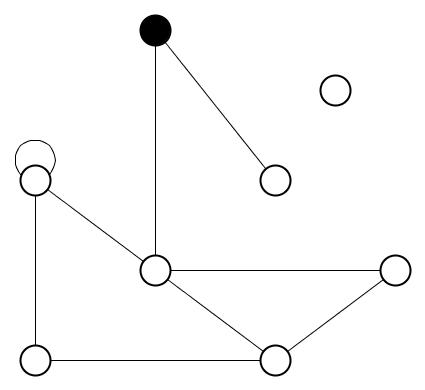
\includegraphics[width=0.5\textwidth]{graph}
 	\caption{Beispiel eines ungerichteten Graphen mit einem Startknoten und einer Schlinge.}
	\label{fig:graph}
\end{figure}
Abbildung~\ref{fig:graph} zeigt ein Beispiel für einen ungerichteten Graphen. Eingezeichnet ist bereits ein Startknoten (schwarzer Knoten) da jede Breitensuche neben dem Graphen einen Start- beziehungsweise Wurzelknoten als Eingabeparameter erwartet. Zusätzlich ist im Graphen eine Schlinge ersichtlich, es sind also auch Kanten zugelassen, bei denen Anfangsknoten gleich Endknoten sind, was innerhalb einer Implementierung der Breitensuche berücksichtigt werden muss. Außerdem kann es sein, dass der Graph nicht zusammenhängend ist. Dabei heißt nach Drmota, Gittenberger, Karigl und Panholzer in~\cite{mathematik} ein ungerichteter Graph \(G\) zusammenhängend, wenn es zwischen je zwei Knoten \(v_{1},v_{2} \in V(G)\) eine Kantenfolge von \(v_{1}\) nach \(v_{2}\) gibt. Liegt ein nicht zusammenhängender Graph vor, kann durch die Breitensuche nur ein Teilgraph beziehungsweise eine sogenannte \textbf{Zusammenhangskomponente} ausgehend vom Startknoten durchsucht werden.\\
Um die Breitensuche zu konkretisieren beziehungsweise besser beschreiben zu können, wird unter anderem der Begriff des Weges und der Distanz zwischen zwei Knoten spezifiziert. Eine Kantenfolge \(e_{1}, e_{2}, ..., e_{k} \in E(G)\) in einem ungerichteten Graphen \(G\) heißt \textbf{Weg}, wenn alle Knoten, die durch diese Kantenfolge durchlaufen werden, voneinander verschieden sind. Während die Länge des Weges mit der Anzahl der Kanten zwischen zwei Knoten gleichzusetzen ist, bezeichnet man die \textbf{Distanz} zweier Knoten  als den kürzesten Weg zwischen diesen. Das Prinzip der Breitensuche impliziert nun, dass zuerst die Knoten mit der Distanz \(d\) besucht werden und erst in Folge die Knoten mit der Distanz \(d+1\). Dadurch wird der Graph durch die Breitensuche in Levels unterteilt, wobei ein \textbf{Level} eine Menge von Knoten definiert, die die selbe Distanz zum Startknoten aufweisen, was in Abbildung~\ref{fig:graph_level} ersichtlich ist. Dabei kann man auch sagen, dass der Knoten die Distanz \(d\) aufweist beziehungsweise zum Level \(d\) gehört. Die größte Distanz zum Startknoten beziehungsweise Wurzelknoten, die ein durch die Breitensuche erreichbarer Knoten aufweist, wird auch als \textbf{Höhe} \(H\) (\textit{height}) des durch die Breitensuche entstandenden Baumes bezeichnet.\\
\begin{figure}[h]
 	\centering
	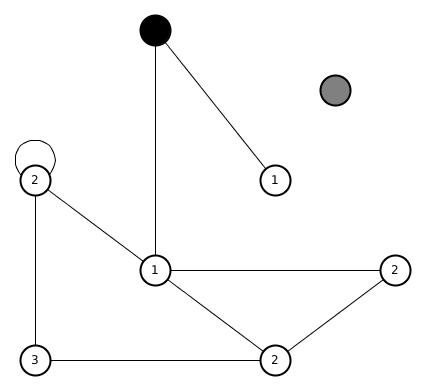
\includegraphics[width=0.5\textwidth]{graph_level}
 	\caption{Nach der Breitensuche ist der Graph in Levels unterteilt. Dies ist ersichtlich an den Distanzen, die in den Knoten eingezeichnet sind. Der graue Knoten entspricht einem nicht besuchten Knoten.}
	\label{fig:graph_level}
\end{figure}
Ausgehend vom Startknoten wurde die Breitensuche auf den Graph von Abbildung~\ref{fig:graph} angewendet. Dadurch wird der Graph in die einzelnen Levels unterteilt, welche aus der Beschriftung der Knoten ersichtlich sind. Der grau hinterlegte Knoten entspricht einem Knoten, der durch die Breitensuche nicht erreicht wurde, also nicht in derselben Zusammenhangskomponente liegt. Die Höhe \(H\) ist gleich dem höchstem Level im Graphen und ist in diesem Fall \(3\).
Es ist auch möglich, andere Informationen als die Distanz in Bezug auf einen Knoten abzuspeichern. Dies wird von vielen unterschiedlichen Applikationen, die die Breitensuche anwenden, erwartet beziehungsweise gefordert. Für unsere Implementierungen ist es Voraussetzung, dass der Vaterknoten für jeden besuchten Knoten abgespeichert wird, damit man am Ende der Breitensuche einen Spannbaum der besuchten Knoten liefern kann. Diese Voraussetzung hat auch unsere Implementierungen stark beeinflusst, da es das Problem der Breitensuche, im Speziellen für den parallelen Fall, aufwendiger macht. Aus Performancezwecken und auch als Beitrag zur Einfachheit und Parallelität sollten zusätzlichen Informationen oder Berechnungen, wenn möglich, beim erstmaligen Besuchen des Knoten durchgeführt werden.
\subsection{Sequentielle Breitensuche}
Nachdem die grundlegenden Bestandteile und Eigenschaften eines Graphen geklärt sind, widmen wir uns weiters dem eigentlichen Thema dieser Arbeit, nämlich der Breitensuche. Auch wenn das Grundkonzept der Breitensuche schon erklärt wurde, zeigt Algorithmus~\ref{fifo} eine klassische sequentielle Variante von Cormen, Leiserson, Rivest und Stein \cite{cormen_introduction_2009}, welche eine Warteschlange (\textit{queue}) verwendet, die im FIFO (\textit{first in first out}) Prinzip arbeitet. Diese Variante der Implementierung gehört zu einer der einfachsten der Breitensuche.
\begin{lstlisting}[caption={Klassische Variante der Breitensuche unter Verwendung einer FIFO Warteschlange als Datenstruktur. Wird auf einem Graph \(G\) mit Startknoten \(s \in V(G)\) angewandt. Der Algorithmus bestimmt die Distanz und den Vaterknoten von denjenigen Knoten, die ausgehend vom Startknoten erreichbar sind.},label=fifo]
$\textbf{SERIAL-BFS-QUEUE}$(G,$s$)
	$\textbf{for}$ each vertex u $\in$ V(G) - {$s$}
		u.d = $\infty$
		u.$\pi$ = NIL
	$s$.d = 0
	$s$.$\pi$ = s
	Q = {$s$}
	$\textbf{while}$ Q $\neq$ $\emptyset$
		u = DEQUEUE(Q)
		$\textbf{for}$ each v $\in$ G.Adj[u]
			$\textbf{if}$ v.d == $\infty$
				v.d = u.d + 1
				v.$\pi$ = u
				ENQUEUE(Q,v)
\end{lstlisting}
Zu Beginn von Algorithmus~\ref{fifo} werden alle Knoten, die in \(V(G)\) enthalten sind, in den Zeilen 2-4 initialisiert. Ein Knoten \(u \in V\) besitzt die Attribute \lstinline{u.d} für die Distanz und \lstinline{u.$\pi$} für den Vaterknoten. Da zu Beginn noch keine Knoten besucht wurden, wird die Distanz \lstinline{u.d} von allen Knoten außer dem Startknoten auf \lstinline{$\infty$} und der Vaterknoten \lstinline{u.$\pi$} auf \lstinline{NIL} gesetzt. Das hat auch folgenden Grund, dass Knoten, die nicht durch die Breitensuche erreicht werden, keine Vaterknoten besitzen, \lstinline{u.$\pi$ = NIL}, und keine gültige Distanz, \lstinline{u.d = $\infty$}, ausgehend vom Startknoten aufweisen.\\
Zeile 5 weist dem Attribut Distanz des Startknotens \(s\) den Wert 0 zu. In Zeile 6 wird der Vaterknoten des Startknotens auf sich selbst gesetzt. In Zeile 7 wird die Warteschlange initialisiert und bekommt als erstes Element den Startknoten. Nun wird die \lstinline{$\textbf{while}$} Schleife von Zeile 8-14 solange ausgeführt, solange es Knoten gibt, die noch nicht besucht wurden, aber vom Startknoten erreichbar sind. Innerhalb der \lstinline{$\textbf{while}$} Schleife wird in Zeile 9 das Element nach dem FIFO Prinzip aus der Warteschlange genommen, das heißt das Element, das zeitlich am längsten in der Warteschlange war. Die \lstinline{$\textbf{for}$} Schleife in den Zeilen 10-14 iteriert über die Nachbarn \lstinline{v $\in$ G.Adj[u]} des aktuellen Knoten \lstinline{u}. Als Nachbar werden folgende Knoten bezeichnet, die adjazent zum jeweiligen Knoten sind, also durch eine Kante verbunden sind. In Zeile 11 wird überprüft, ob der Knoten \lstinline{v} noch nicht besucht wurde, was mittels \lstinline{$\textbf{if}$} Bedingung
\lstinline{v.d == $\infty$} geprüft wird. Ist dies der Fall, wird \lstinline{v.d} auf \lstinline{u.d + 1} gesetzt und \lstinline{u} wird als Vater in \lstinline{v.$\pi$} gekennzeichnet. Danach wird der Knoten \lstinline{v} in die Warteschlange aufgenommen. Der Algorithmus endet, wenn bei der Überprüfung der Bedingung in Zeile 8 keine Elemente in der Warteschlange vorhanden sind, was bedeutet, dass alle erreichbaren Knoten besucht wurden und die Schleife abbricht.\\
Dadurch dass jedem besuchten Knoten \lstinline{v} mit \lstinline{v.$\pi$} der Vaterknoten zugewiesen wird, entsteht durch die Breitensuche ein Subgraph von \(G\) der Vaterknoten, definiert durch \(G_{\pi} = (V_{\pi}, E_{\pi})\), wobei \(V_{\pi} = \{v \in V : v.\pi \neq\) \lstinline{NIL}\(\}\) und \(E_{\pi} = \{\{v.\pi,v\} : v \in V_{\pi} - s\}\). Beim Subgraph \(G_{\pi}\) handelt es sich um einen Baum (\textbf{\textit{Breadth-First Tree}}), der alle Knoten \(V_{\pi} \) enthält, die vom Startknoten \(s\) erreichbar sind. Da es sich um einen Baum handelt, existiert für alle Knoten \(v \in V_{\pi}\) im Subgraphen \(G_{\pi}\) genau ein Pfad von \(s\) nach \(v\), der gleichzeitig auch der kürzeste Pfad von \(s\) nach \(v\) in \(G\) ist.
\subsection{Analyse von Algorithmen}
Um Vorherzusagen, wie viele Ressourcen ein Algorithmus benötigen wird, ist die Analyse eines Algorithmus entscheidend. Dabei ist für uns die Ressource \textbf{Laufzeit} maßgebend. Falls man mehrere Algorithmen zur Lösung eines Problems zur Verfügung hat, entscheidet man sich häufig für den Algorithmus mit der besten Laufzeit.\\
Um einen Algorithmus maschinenunabhängig analysieren zu können, macht man Gebrauch vom RAM (\textit{random-access machine}) Modell. Dieses abstrakte Rechnermodell hat einen einzigen Prozessor und Instruktionenen werden sequentiell ausgeführt. Folgende Annahmen werden getroffen:
\begin{itemize}
	\item{Eine einfache Operation wird in einem Schritt ausgeführt.}
	\item{Subroutinen und Schleifen sind keine einfachen Operationen.}
	\item{Der Speicher ist unbegrenzt, ein Speicherzugriff benötigt einen Schritt.}
\end{itemize}
Die Laufzeit des Algorithmus ist nun die Anzahl der benötigten Schritte, die abhängig von der Länge \(n\) der Eingabe ist und für größer werdende \(n\) asymptotisch unter Verwendung der Landau-Notation abgeschätzt wird. Eine ausführliche und weiterführende Beschreibung der Analyse von Algorithmen ist in \cite{cormen_introduction_2009} von Cormen et al. zu finden.\\
Um die sequentielle Breitensuche im RAM Modell zu analysieren, ist es nun entscheidend von welchen Eingaben die Laufzeit abhängt. Es stellt sich heraus, dass die Anzahl der Knoten \(n = |V(G)|\) und der Kanten \(m = |E(G)|\) eines Graphen die Laufzeit der Breitensuche beeinflussen. Algorithmus~\ref{fifo} weist eine Laufzeit von \($O$(n + m)\) auf, da alle Knoten und damit auch alle Kanten genau einmal besucht werden. Die Anzahl der Iterationen, Zeile 8-14, ist dabei gebunden an die Anzahl der Knoten \(|V(G)|\) und innerhalb jedes Knoten werden all seine Kanten, Zeile 10-14, angesehen. 
\section{Parallele Breitensuche}
\label{parallel}
In diesem Kapitel werden wir parallele Algorithmen für die Breitensuche vorstellen, die den Graphen parallel traversieren und im Vergleich zur sequentiellen Variante einen Speedup erzielen. Der \textbf{Speedup}-Begriff, wie durch Rauber und Rünger~\cite{rauber} definiert, wird als Maß für den relativen Geschwindikeitsgewinn herangezogen. Der Speedup \(S_{p}(n)\) ist definiert als
\begin{equation}
	S_{p}(n) = \frac{T^{*}(n)}{T_{p}(n)}
\end{equation}
Dabei ist \(T^{*}(n)\) die Laufzeit einer optimalen sequentiellen Implementierung und \(T_{p}(n) \) die Laufzeit eines parallelen Programmes. Hier steht \(p\) für die Anzahl der zur Verfügung stehenden Prozessoren zur Lösung eines Problems der Größe \(n\). Es gilt \(S_{p}(n) \leq p\). Wäre \(S_{p}(n) \geq p\), könnte man einen sequentiellen Algorthmus finden, der schneller als der für die Berechnung des Speedups verwendete ist.\\
Neben der Laufzeit und des Speedups eines parallelen Programms spielt in unserer Analyse von parallelen Lösungen noch ein dritter Faktor eine wichtige Rolle, nämlich die Kosten. Die \textbf{Kosten} eines parallelen Programms sind nach Rauber und Rünger \cite{rauber} definiert als
\begin{equation}
	C_{p}(n) = T_{p}(n) \cdot p
 \end{equation}
und ist die von allen Prozessoren ausgeführte Arbeit. Unser Ziel in Bezug auf die Kosten ist es, ein paralleles Programm zu finden, dass \textbf{kostenoptimal} beziehungsweise annähernd kostenoptimal ist, also bei dem bei der Verwendung asymptotischer Laufzeiten gilt \(C_{p}(n) = T^{*}(n)\). Das heißt es sollen vom parallelen Programm insgesamt genauso viele Operationen ausgeführt werden wie von einem optimalen sequentiellen Verfahren.
\subsection{Erste Überlegungen}
Nachdem beschrieben wurde, wie ein paralleles Programm in unserer Arbeit bewertet wird, auch in Bezug auf das sequentielle Verfahren, wenden wir uns wieder dem eigentlichen Thema zu, der Breitensuche und deren Parallelisierung. Es ist bei vielen Problemen schwierig einen sequentiellen Algorithmus mit nur wenigen Änderungen in einen parallelen umzusetzen. Oft muss man eine andere Sicht auf das zu lösende Problem bekommen und eine ähnliche oder andere Lösung heranziehen, bei der eine parallele Umsetzung besser möglich ist. Ein Beispiel dafür ist Algorithmus~\ref{fifo}.  Dieser Algorithmus zur Lösung der Breitensuche ist schwierig zu parallelisieren, da die FIFO Warteschlange ein Hindernis für die Parallelisierung auf Rechnern mit physikalisch verteiltem Speicher darstellt, falls man diese im parallelen Algorithmus synchronisiert halten will. Ein ausführlichere Beschreibung liefert hierbei Leiserson und Schardl~\cite{leiserson}.\\
Aus diesem Grund geben wir noch einen weiteren sequentiellen Algorithmus durch Algorithmus~\ref{stacks} an, der anstatt der FIFO Warteschlange zwei Stapelspeicher (\textit{stacks}) verwendet, wodurch ein level-basiertes Durchsuchen des Graphen, wie in Abbildung~\ref{fig:graph_level}, ersichtlicher wird. Mit Hilfe von Algorithmus~\ref{stacks} ist es einfacher, einen parallelen Algorithmus abzuleiten. Dieser Algorithmus wird auch von Buluç und Madduri~\cite{buluc} als Basis für deren Arbeit zur parallelen Breitensuche verwendet und ist auch in deren Arbeit abgebildet.
\begin{lstlisting}[caption={Eine weitere sequentielle Variante der Breitensuche unter Verwendung von zwei Stacks \lstinline{FS} und \lstinline{NS} als Datenstrukturen. Dieser Algorithmus liefert das gleiche Ergebnis wie Algorithmus~\ref{fifo} und hat auch die gleiche Laufzeit wie dieser, ermöglicht jedoch eine bessere Sicht auf das level-basierte Durchsuchen des Graphen, was das Ableiten eines parallelen Algorithmus einfacher macht.},label=stacks]
$\textbf{SERIAL-BFS-STACKS}$(G,$s$)
	$\textbf{for}$ each vertex u $\in$ V(G) - {$s$}
		d[u] = $\infty$
		$\pi$[u] = NIL
	d[s] = 0
	$\pi$[s] = s
	level = 1
	FS = {s}
	NS = $\emptyset$
	$\textbf{while}$ FS $\neq$ $\emptyset$
		$\textbf{for}$ each u $\in$ FS
			$\textbf{for}$ each v $\in$ G.Adj[u]
				$\textbf{if}$ d[v] == $\infty$
					d[v] = level
					$\pi$[v] = u
					NS = NS $\cup$ {v}
		FS = NS
		NS = $\emptyset$
		level = level + 1
\end{lstlisting}
Algorithmus~\ref{stacks} ist sehr ähnlich zu Algorithmus~\ref{fifo}. Es werden jedoch zwei Datenstrukturen zur Durchsuchung des Graphen benötigt und es gibt eine weitere verschachtelte Schleife in Zeile 11. Bei den zwei Datenstrukturen handelt es sich um \lstinline{FS} (\textit{frontier stack}), der Stapelspeicher, wo die Knoten des aktuellen Levels gespeichert sind, und \lstinline{NS} (\textit{newly-visited stack}), der Stapelspeicher, wo die neu besuchten Knoten gespeichert werden, also die Knoten, die ein um eins höheres Level haben als die Knoten in \lstinline{FS}. Einen Unterschied gibt es auch in der Abspeicherung der Distanz \(d\) und des Vaterknotens \(\pi\) zu jedem Knoten. Im Gegensatz zu Algorithmus~\ref{fifo} werden diese Informationen nicht direkt beim Knoten über ein Attribut abgespeichert, sondern in einer eigenen Datenstruktur \lstinline{d[1..n]} und \lstinline{$\pi$[1..n]}. In diesem Fall handelt es sich um Arrays der Länge \lstinline{n}, wobei es sich bei \lstinline{n} um die Anzahl der Knoten handelt.\\
Nach der Initialisierung wird die \lstinline{$\textbf{while}$} Schleife von Zeile 10-19 solange ausgeführt bis es keine neu besuchten Knoten gibt, also keine weiteren Knoten ausgehend vom Startknoten \lstinline{$s$} erreicht werden können. In den Zeilen 11-16 wird mittels \lstinline{$\textbf{for}$} Schleife über alle Knoten des aktuellen Levels iteriert. Durch die Bedingung in Zeile 10 muss zumindest ein Element \lstinline{u} in \lstinline{FS} enthalten sein. Über die Nachbarn des Knoten \lstinline{u} in Zeile 12-16 wird genauso iteriert wie in Algorithmus~\ref{fifo}, außer dass hier die Nachbarn \lstinline{v}, die zuvor noch nicht besucht wurden, also \lstinline{d[v] == $\infty$}, im Stapelspeicher \lstinline{NS} abgelegt werden. Ebenfalls sehr entscheidend für diesen Algorithmus ist, dass nachdem alle Knoten des aktuellen Levels abgearbeitet wurden, der Stapelspeicher \lstinline{FS} die Elemente von \lstinline{NS} übernimmt und \lstinline{NS} geleert wird. \lstinline{FS} hat also alle Knoten nun gespeichert, die zuvor in Zeile 14-16 neu besucht wurden. Danach wird der Wert von \lstinline{level}, der den neu besuchten Knoten durch \lstinline{d[v] = level} in Zeile 14 zugewiesen wird, um eins erhöht und die nächste Iteration mit den neu besuchten Knoten startet.\\
Als Ausgabe erhalten wir genauso wie bei Algorithmus~\ref{fifo} einen Breadth-First Tree. Die Laufzeit von Algorithmus~\ref{stacks} ist genauso wie bei Algorithmus~\ref{fifo} \($O$(n + m)\), wobei die Anzahl der Iterationen von der \lstinline{$\textbf{while}$} Schleife von Zeile 10-19 gebunden ist an die Länge des längsten Pfades vom Startknoten \(s\) zu einem erreichbaren Knoten im Graphen \(G\), was der Höhe \(H\) des Subgraphen \(G_{\pi}\) entspricht.\\
Anhand dieser Überlegungen gibt es nun unterschiedliche Wege die Breitensuche zu parallelisieren. Wie schon durch Buluç und Madduri~\cite{buluc} spezifiert, gibt es zwei grundlegende Varianten, wie man dieses Problem parallelisiert, nämlich durch Zerlegung beziehungsweise Aufteilung des Graphen auf die zur Verfügung stehenden Prozessoren. Natürlich hängt diese Zerlegung auch von der Repräsentation des Graphen in der Implementierung ab, womit wir uns aber erst in Kapitel~\ref{sec:details} genauer beschäftigen werden. Vorerst ist nur die Idee der Zerlegung wichtig. Wir gehen davon aus, dass die Knoten des Graphen durchgehend nummeriert sind und dass wir mit jeder Knotennummer direkt auf die Kanten dieses Knoten zugreifen können.
\begin{itemize}
	\item{Eindimensionale (\textbf{1D}) Zerlegung des Graphen bedeutet nun, dass man die Knoten des Graphen \(V(G)\) auf die Prozessoren so aufteilt, dass, wenn \(n = |V(G)|\), jeder Prozessor in Besitz von \(n / p\) Knoten ist, wobei \(p\) die Anzahl der verfügbaren Prozessoren darstellt. Zusätzlich besitzt jeder Prozessor lokal die Kanten, die mit einem auf dem Prozessor gespeicherten Knoten verbunden sind, also jede Kante \(e = \{v_{1},v_{2}\}, e \in E(G)\), wo entweder \(v_{1}\) oder \(v_{2}\) ein lokaler Knoten des Prozessors ist, da es sich um einen ungerichteten Graphen handelt.}
	\item{Bei der zweidimensionalen (\textbf{2D})  Zerlegung werden nicht nur die Knoten unter den Prozessoren aufgeteilt, sondern es werden auch die zu den Knoten zugehörigen Kanten unter mehreren Prozessoren aufgeteilt. Das heißt es kann sein, dass mehrere Prozessoren die gleiche Knotenmenge besitzen, jedoch unterschiedliche Kanten zu diesen Knoten.}
\end{itemize}
Diese Zerlegungen lassen sich sehr gut mit einer Adjazenzmatrix darstellen, es ist jedoch nicht notwendig auch eine Matrix als Graphrepräsentation in der Implementierung zu verwenden, diese Repräsentation soll nur zum Verständnis beitragen.
\begin{figure}[h]
    \centering
    \begin{subfigure}[b]{0.45\textwidth}
        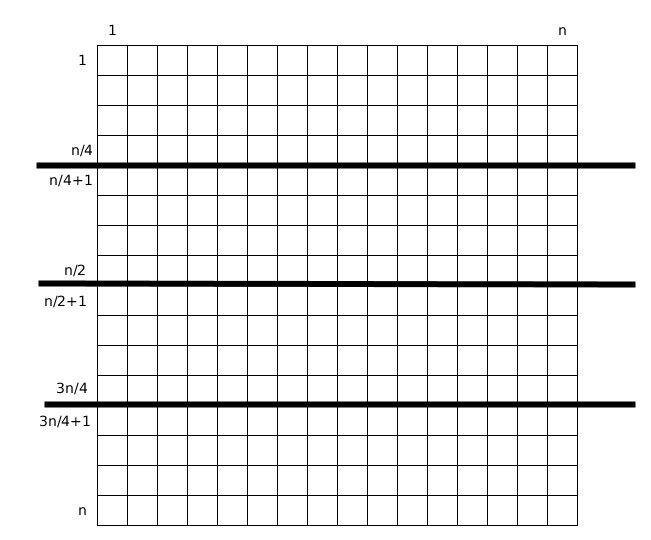
\includegraphics[width=0.9\textwidth]{eindim}
        \caption{eindimensional}
        \label{fig:eindim}
    \end{subfigure}
   \qquad
    \begin{subfigure}[b]{0.47\textwidth}
        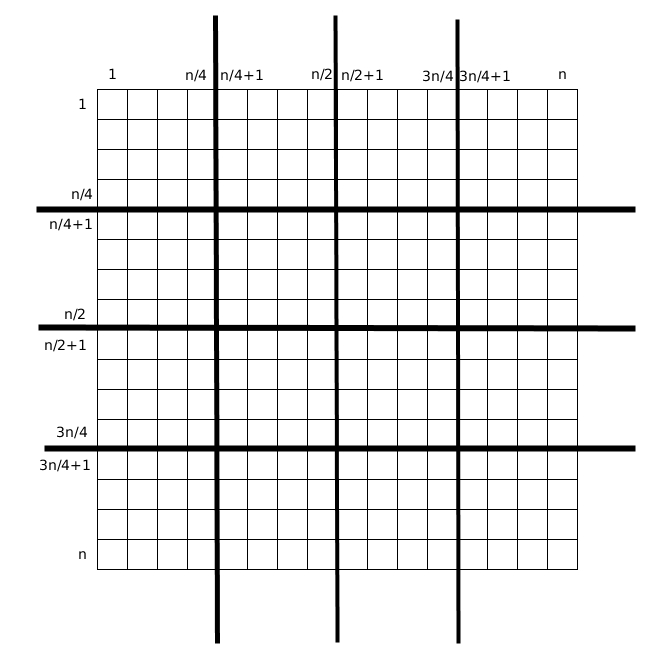
\includegraphics[width=0.9\textwidth]{zweidim}
        \caption{zweidimensional}
        \label{fig:zweidim}
    \end{subfigure}
    \caption{Es ist möglich, den Graphen ein- oder zweidimensional zu zerlegen. Diese abstrakte Darstellung einer Adjazenzmatrix in Abbildung~\ref{fig:eindim} zeigt, dass im eindimensionalen Fall die Zerlegung nur auf einer Achse erfolgt, im zweidimensionalen Fall in Abbildung~\ref{fig:zweidim} auf zwei Achsen.}
\label{fig:zerlegung}
\end{figure}
Abbildung~\ref{fig:zerlegung} zeigt die Zerlegung des Graphen im ein- und zweidimensionalen Fall. Repräsentiert wird der Graph durch eine Adjazenzmatrix mit \(n = 16\) Knoten. Auf beiden Achsen sind die Knoten eingetragen und jeder Eintrag beziehungsweise jede Zelle der Matrix repräsentiert eine Kante. Im eindimensionalen Fall heißt das, dass die Knoten, die auf der vertikalen Achse eingetragen sind, unter den Prozessoren aufgeteilt werden, was durch die Linien dargestellt ist. In diesem Fall handelt es sich um 4 Prozessoren, die die Matrix untereinander aufteilen. Der Prozessor speichert zu den Knoten, über die er verfügt, alle Kanten zu diesen Knoten ab, was dadurch dargestellt ist, dass der Bereich des Prozessors die gesamten Zeilen zu den Knoten umfasst. Das bedeutet auch, da wir mit ungerichteten Kanten arbeiten, dass jede Kante zweimal abgespeichert wird, jeweils einmal bei jedem Endknoten dieser Kante. Im Gegensatz dazu wird bei der zweidimensionalen Zerlegung auch die horizontale Achse auf mehrere Prozessoren aufgeteilt, wodurch es, wie schon weiter oben erwähnt, der Fall ist, dass sich mehrere Prozessoren die gleiche Knotenmenge teilen, aber unterschiedliche Kanten zu diesen Knoten abspeichern beziehungsweise behandeln. In Abbildung~\ref{fig:zweidim} würden sich 16 Prozessoren den Graphen untereinander aufteilen. Die obersten vier Bereiche der Abbildung sind die Bereiche von 4 Prozessoren. Diese Prozessoren sind für die gleichen Knoten verantwortlich, also für die Knoten 1 bis 4. Jedoch speichert der erste Prozessor die Kanten, die von den Knoten 1 bis 4 ausgehen, und zu den Knoten 1 bis 4 gehen. Der zweite Prozessor speichert die Kanten, die auch von den Knoten 1 bis 4 ausgehen, jedoch zu den Knoten 5 bis 8 verlaufen. Die anderen zwei Prozessoren decken dann die restlichen Kanten ausgehend von den Knoten 1 bis 4 ab.\\
Ausgehend von der level-basierten sequentiellen Breitensuche, dargestellt durch Algorithmus~\ref{stacks}, und der eindimensionalen Zerlegung des Graphen, werden wir in den nächsten Kapiteln zwei Algorithmen zur parallelen Breitensuche abstrakt veranschaulichen. Grundlegender Unterschied dieser zwei Algorithmen ist die Synchronisation zwischen den Prozessoren, also welche Daten werden wie synchronisiert. Außerdem liegen Unterschiede darin, wieviel die Prozessoren über den Gesamtzustand des Systems wissen, also zum Beispiel ob Knoten, die anderen Prozessoren zugeordnet sind, bereits besucht wurden und deshalb im nächsten Level nicht mehr berücksichtigt werden müssen. Wichtig ist jedoch, dass beide Algorithmen mit einer 1D Zerlegung des Graphen arbeiten und als Ausgabe einen Breadth-First Tree haben müssen. Falls dieser Breadth-First Tree in einem Array abgespeichert ist, bezeichnen wir dieses Array auch als \textbf{\textit{Parent Array}}.  Dabei wollen wir festlegen, dass dieses Parent Array am Ende des Algorithmus nicht unbedingt auf einem Prozessor liegen muss, sondern auf den arbeitenden Prozessoren verteilt sein kann. Details über die Implementierungen und welche Auswirkungen diese Unterschiede auf die Laufzeit haben, sind in Kapitel~\ref{sec:details} beziehungsweise Kapitel~\ref{sec:analysechapter} zu finden.
\subsection{Paralleler BFS mit Allreduce Kommunikation}
\label{sec:bfs_allreduce}
Die Idee hinter diesem Algorithmus war neben der eindimensionalen Zerlegung des Graphen und damit parallelen Abarbeitung der Levels, dass die Prozessoren mehr Informationen über die anderen Prozessoren haben und den zugehörigen Knoten. Bei vielen parallelen Algorithmen der Breitensuche, wie auch beim Algorithmus in Kapitel~\ref{sec:bfs_alltoall} ist es so, dass die Prozessoren nur Informationen über die lokal gespeicherten Knoten besitzen und anhand dieser Informationen Entscheidungen treffen müssen, wodurch es zu einen erhöhten Kommunikationsaufwand zwischen den Prozessoren kommen kann. Zum Beispiel ist es einem Prozessor, der die Nachbarn eines neu besuchten Knoten durchläuft, bei diesen Algorithmen nicht oder nur begrenzt bekannt, ob ein Knoten, der nicht zu den lokalen gehört, bereits besucht wurde, da dies nur der Prozessor weiß, dem der Knoten zugeteilt ist. Deshalb muss jedes Mal bei einem für einen Prozessor fremden Knoten, zwischen den Prozessoren kommuniziert werden, ob dieser Knoten bereits in einem vorherigen Level besucht wurde.\\
Aufgrund dieser Tatsache wird bei unserem ersten Algorithmus eine Datenstruktur zwischen den Prozessoren synchron gehalten, die über alle Knoten des Graphen die Information besitzt, ob ein Knoten besucht wurde oder nicht. Falls wir uns also gerade im Level \(d\) befinden, weiß jeder Prozessor welche Knoten im Graphen bis einschließlich zum Level \(d-1\) besucht wurden. Dazu verwenden wir als Datenstruktur ein Array \lstinline{a[1..n]}, wie in Algorithmus~\ref{par_allvisited} ersichtlich, das zu jedem Knoten die Information speichert, ob dieser Knoten bisher besucht wurde oder nicht. Dies stellen wir durch Abspeichern der Werte 0 (nicht besucht) und 1 (besucht) in \lstinline{a[k]} zu jedem Knoten \(k \in V(G)\) sicher. Da wir anhand dieser Datenstruktur nur wissen, welche Knoten bis einschließlich des letzten Levels besucht wurden, jedoch nicht, welche davon noch nicht von den zuständigen Prozessoren bearbeitet wurden, braucht jeder Prozessor noch ein zweites Array \lstinline{v[1..n/p]}, welches zu jedem lokalen Knoten abspeichert, 0 oder 1, ob dieser Knoten lokal behandelt wurde und damit auch die Nachbarn dieses Knoten besucht wurden. Dieses Hilfsarray hat die Länge \lstinline{n/p}, da jeder Prozessor für \lstinline{n/p} Knoten verantwortlich ist. Dabei ist \lstinline{p} die Anzahl der zur Verfügung stehenden Prozessoren. Zu beachten ist auch, dass alle Prozessoren ein Parent Array \lstinline{$\pi$} der Länge \(n\) besitzen. Falls also ein Knoten \(x\) ausgehend von Knoten \(y\) zum ersten Mal besucht wird, dann trägt der Prozessor, der für \(y\) verantwortlich ist, den Knoten \(y\) als Vater von \(x\) ein, also \lstinline{$\pi$[x] = y}, wobei es sich bei \lstinline{$\pi$}, um das auf dem Prozessor lokal gespeicherte Parent Array handelt.
\begin{lstlisting}[caption={Die Prozedur \lstinline{PARALLEL-BFS-ALLREDUCE} wird von allen verfügbaren Prozessoren parallel aufgerufen. Nach jeder Abarbeitung eines Levels findet durch die \lstinline{ALLREDUCE} Operationen eine sogenannte Barrier-Synchronisation statt, bei der zwischen den Prozessoren ausgetauscht wird, ob es überhaupt einen neu besuchten Knoten gibt (\lstinline{isNewLevel}), beziehungsweise wird das Array \lstinline{a} synchronisiert.},label=par_allvisited]
$\textbf{PARALLEL-BFS-ALLREDUCE}$($G_{p}$,s)
	$\textbf{for}$ 1 $\leq$ i $\leq$ n $\textbf{do}$
		a[i] = 0
		$\pi$[i] = NIL
	$\textbf{for}$ 1 $\leq$ i $\leq$ n/p $\textbf{do}$
		v[i] = 0
	a[s] = 1
	isNewLevel = 1
	$\pi$[s] = s
	$\textbf{while}$ (isNewLevel == 1)
		isNewLevel = 0
		$a_{p}$ = a[n/$\textit{p}$*$\textit{rank}$+1..n/$\textit{p}$*($\textit{rank}$+1)]
		FS = $\textit{GETNEWVISITED}$($a_{p}$,v)
		$\textbf{for}$ each u $\in$ FS
			v[$\textit{LOCAL}$(u)] = 1
			$\textbf{for}$ each w $\in$ $G_{p}$.Adj[u]
				$\textbf{if}$ a[w] == 0
					a[w] = 1
					$\pi$[w] = u
					isNewLevel = 1
		ALLREDUCE(isNewLevel,OR)
		ALLREDUCE(a,OR)
	REDUCE($\pi$, MAXIMUM, $p_{0}$)
\end{lstlisting}
Um den Algorithmus besser zu strukturieren, verwenden wir das \textbf{BSP-Modell} (\textit{bulk synchronous parallel}), das eine Abstraktion eines Rechners mit physikalisch verteiltem Speicher darstellt, so wie von Rauber und Rünger in \cite{rauber} beschrieben. Grundlegend für dieses Modell, wie in Abbildung~\ref{fig:bsp} ersichtlich, ist, dass eine Berechnung (Ergebnis eines Algorithmus) aus einer Folge von \textbf{Superschritten} besteht. In jedem Superschritt führt jeder Prozessor lokale Berechnungen durch und am Ende findet eine Barrier-Synchronisation statt, die durch globale Kommunikationoperationen bewerkstelligt wird. Wichtig in diesem Modell ist jedoch, dass die Barrier-Synchronisation für alle Prozessoren zum gleichen Zeitpunkt stattfindet und dass die verschickten Daten erst im nächsten Superschritt verwendet werden.
\begin{figure}[h]
 	\centering
	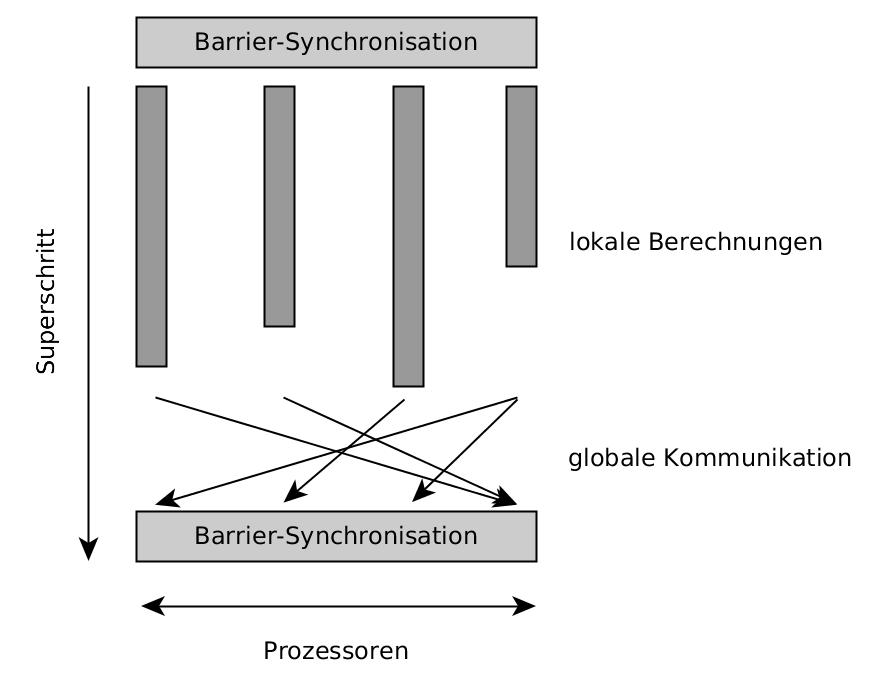
\includegraphics[width=0.5\textwidth]{bsp}
 	\caption{Beim BSP-Modell entsteht ein Resultat eines Algorithmus aus einer Vielzahl von sogenannten Superschritten. Man kann sagen, dass ein Superschritt wiederum aus mehreren Schritten besteht, nämlich aus den lokalen Berechnungen der beteiligten Prozessoren, der globalen Kommunikationsoperationen zwischen den Prozessoren beziehungsweise dem Austausch von Daten und der Barrier-Synchronisation, die durch diese Kommunikationsoperationen bewerkstelligt wird. Wichtig für dieses Modell ist, dass die Prozessoren jene Daten in den lokalen Berechnungen verwenden, die sie aus der Kommunikation des letzten Superschritts erhalten haben.}
	\label{fig:bsp}
\end{figure}
In Algorithmus~\ref{par_allvisited} wird in einem Superschritt ein Level bearbeitet und entspricht einer Iteration der \lstinline{$\textbf{while}$} Schleife von Zeile 10-22.  Jeder Prozessor führt innerhalb dieses Superschrittes seine lokalen Berechnungen durch, bis am Ende die Barrier-Synchronisation durch die \lstinline{ALLREDUCE} Operationen durchgeführt wird.\\
Jeder Prozessor ruft die Prozedur \lstinline{PARALLEL-BFS-ALLREDUCE} auf und hat als Eingabe einen Teilgraphen \lstinline{$G_{p}$} und den Startknoten \lstinline{s}. Beim Teilgraphen \lstinline{$G_{p}$} handelt es sich um den eindimensional zerlegten Graphen. Das heißt jeder Prozessor besitzt \(n/p\) Knoten, welche durch eine Identifikationsnummer eindeutig gekennzeichnet sind, und alle Kanten zu den zugehörigen \(n/p\) Knoten. Dabei können wir davon ausgehen, dass der erste Prozessor die ersten \(n/p\) Knoten zugeteilt bekommt, der zweite die zweiten \(n/p\) Knoten und so weiter. Zu Beginn findet wie bei den vorherigen Algorithmen eine Initialisierung der Datenstrukturen und Variablen statt. Der Startknoten \lstinline{s} wird im Array \lstinline{a} gesetzt. Außerdem brauchen wir eine zusätzliche Variable \lstinline{isNewLevel}, die die Information speichert, ob im letzten Superschritt zumindest ein Knoten besucht wurde. Diese Variable ist notwendig, da die Prozessoren anhand der Informationen der Arrays \lstinline{a} und \lstinline{v} nur herausfinden können, ob ein lokaler Knoten neu besucht wurde, nicht aber ob ein Knoten eines anderen Prozessors neu besucht wurde. Diese Variable wird am Ende jedes Superschrittes synchronisiert und nimmt den Wert 0 in Zeile 21 an, falls kein neuer Knoten innerhalb des aktuellen Superschritt hinzugekommen ist. In Zeile 12 wird durch \lstinline{a[n/$\textit{p}$*$\textit{rank}$+1..n/$\textit{p}$*($\textit{rank}$+1)]} der Teil vom Array \lstinline{a} herausgenommen, der die Knoten enthält, für die der jeweilige aufrufende Prozessor zuständig ist. Mithilfe dieses Ausschnitts \lstinline{$a_{p}$} und des Arrays \lstinline{v}, die jeweils eine Länge von \(n/p\) haben, können nun mit der Funktion \lstinline{GETNEWVISITED} die Knoten herausgefiltert werden, die im letzten Superschritt neu besucht worden sind. Die Abarbeitung der zu bearbeitenden Knoten ist sehr ähnlich zu Algorithmus~\ref{stacks}, außer dass zusätzlich die Variable \lstinline{isNewLevel} benötigt wird und auf 1 gesetzt wird, sobald ein neuer Knoten besucht wird. Auch muss auf das Array \lstinline{v} mittels der Funktion \lstinline{$\textit{LOCAL}$} zugegriffen werden, da die Identifikationsnummern der Knoten von \(1\) bis \(n\) gehen, jedoch dieses Array eine Größe von \(n/p\) hat, da Informationen nur über die lokalen Knoten gespeichert wird. Deshalb muss der lokale Index für dieses Array berechnet werden, was jedoch nicht viel mehr als eine Modulo Operation ist.\\
Am Ende des Algorithmus findet die Barrier-Synchronisation statt, die mittels \lstinline{ALLREDUCE} Operationen ausgeführt wird. Um die \lstinline{ALLREDUCE} Operation zu erklären, werden wir zuerst auf die Operation \lstinline{REDUCE} eingehen, da man sagen kann, dass \lstinline{ALLREDUCE} in gewissen Sinne eine Erweiterung dieser Operation ist. Bei \lstinline{REDUCE} handelt es sich um eine Akkumulationsoperation oder auch globale Reduktionsoperation, bei der jeder beteiltigte Prozessor Daten zur Verfügung stellt, die mittels einer binären Operation verknüpft werden. Das Ergebnis erhält dann ein definierter Wurzelprozessor. \lstinline{ALLREDUCE} ist eine Multi-Akkumulationsoperation, bei der man sagen kann, dass jeder beteiligte Prozessor eine Einzelakkumulationsoperation ausführt. Einfach ausgedrückt stellt also jeder Prozessor ein Datum zur Verfügung, das heißt es gibt bei \(p\) Prozessoren \(p\) Daten. Diese Daten werden dann mit einer definierten binären Operation zu einem Datum verknüpft und an alle Prozessoren gesendet. Es erhalten somit alle Prozessoren das selbe Ergebnis.\\
Für die Barrier-Synchronisation in Algorithmus~\ref{par_allvisited} wird sowohl \lstinline{isNewLevel} als auch das Array \lstinline{a} synchronisiert. Es werden bei der \lstinline{ALLREDUCE} Operation von jedem Prozessor die Daten \lstinline{isNewLevel} beziehungsweise \lstinline{a} herangenommen und zu einem einzigen Datum verknüpft. Damit keine Information verloren geht, also eine gesetzte 1 entweder in \lstinline{isNewLevel} oder an einer bestimmten Position von \lstinline{a} auch durch die \lstinline{ALLREDUCE} Operation im Ergebnis gesetzt bleibt, kommt nur eine binäre Operation für die Verknüpfung in Frage, nämlich die Operation \lstinline{OR}.\\
Die Schleife von Zeile 10-22 bricht an dem Punkt ab, bei dem kein einziger neuer Knoten von einem Prozessor besucht wird, also die Variable \lstinline{isNewLevel} den Wert 0 annimmt. Da nun ein \textit{Parent Array} \lstinline{$\pi$} als Ergebnis vorhanden ist, dieses jedoch noch auf den einzelnen Prozessoren verteilt ist oder anders gesagt jeder Prozessor nur einen Teil des \textit{Breadth-First Trees} besitzt, wird dieses per \lstinline{REDUCE} Operation verknüpft und das Ergebnis an den Wurzelprozessor \lstinline{$p_{0}$} geliefert. Als binäre Verknüpfungsoperation haben wir \lstinline{MAXIMUM} gewählt, da es sein, dass es mehrere Väter zu einem bestimmten Knoten gibt und der Knoten gewählt wird, der die höhere Identifikationsnummer besitzt. Dieser Fall kann auftreten, wenn ein bestimmter Knoten im gleichen Level von mehrereren Vaterknoten zum ersten Mal besucht wird und diese Vaterknoten, wenn diese zu unterschiedlichen Prozessoren gehören, nicht wissen, dass dieser Knoten gleichzeitig auch von Knoten anderen Prozessoren besucht wird. Dadurch können sich mehrere Knoten als Vater zu denselben Knoten in unterschiedliche lokale Versionen von \lstinline{$\pi$} eintragen.
\begin{table}[h]
\centering
\label{tbl:allreduce}
\begin{tabular}{lcl}
$P_{0}$ : $x_{0}$     		& \multirow{4}{*}{$\Rightarrow$} 	& $P_{0}$ : $x_{0}$ + $x_{1}$ + ... + $x_{p-1}$ \\
$P_{1}$ : $x_{1}$     		&                                 						& $P_{1}$ : $x_{0}$ + $x_{1}$ + ... + $x_{p-1}$ \\
...         			&                                 									& ... \\
$P_{p-1}$ : $x_{p-1}$ 	&                                 						& $P_{p-1}$ : $x_{0}$ + $x_{1}$ + ... + $x_{p-1}$
\end{tabular}
\caption{Die Tabelle, wie sie auch von Rauber und Rünger~\cite{rauber} verwendet wird, zeigt das Resultat der \lstinline{ALLREDUCE} Operation. Jeder Prozessor stellt jeweils ein Datum $x$ zur Verfügung. Diese Daten werden per \lstinline{ALLREDUCE} Operation oder genauer gesagt anhand der binären Operation $+$ zu einem Datum verknüpft und an die beteiligten Prozessoren gesendet.}
\end{table}
\subsection{Paralleler BFS mit All-to-all Kommunikation}
\label{sec:bfs_alltoall}
Im Gegensatz zu Algorithmus~\ref{par_allvisited} setzen wir beim Algorithmus in diesem Kapitel voraus, dass die einzelnen Prozessoren nur über die zugewiesenen Knoten Informationen speichern müssen und dadurch weniger über den Gesamtzustand, also über die nicht zugewiesenen Knoten, wissen. Mit Informationen meinen wir in unserem Fall, ob ein Knoten bereits bearbeitet wurde und um welche Vaterknoten es sich handelt. Ausgehend von diesem Wissen kann es bei so einem Ansatz vorkommen, dass wenn ein fremder Knoten neu besucht wird, dass der zugehörige Prozessor jedes Mal darüber informiert werden muss und dieser dann im nächsten Level überprüft, ob er diesen Knoten schon bearbeitet hat. Dadurch kann es sein, dass in jedem Level der Breitensuche zwischen den Prozessoren Informationen über Knoten ausgetauscht werden müssen, obwohl diese Knoten bereits besucht und bearbeitet sind, was natürlich zu Redundanzen in der Kommunikation führt.\\
Bei diesem Algorithmus arbeiten wir wieder mit den zwei Stacks \lstinline{FS} und \lstinline{NS}, ähnlich wie sie bei der sequentiellen Breitensuche in Algorithmus~\ref{stacks} verwendet wurden. Jeder Prozessor hat dabei einen eigenen Stack \lstinline{FS}, den er in jedem Level abarbeiten muss und der jene Knoten enthält, die im letzten Level von einem beliebigen Prozessor besucht wurden und die diesem Prozessor zugehörig sind. Im Stack \lstinline{FS} können auch Knoten enthalten sein, die schon von diesem Prozessor bearbeitet wurden, jedoch diesmal durch eine andere Kante im Graphen besucht wurden. Diese Knoten ignoriert der Prozessor und geht zum nächsten Knoten im Stack über. Außerdem ist es für einen Prozessor nicht ausreichend, wenn er nur einen Stack \lstinline{NS} anlegt, der die neu besuchten Knoten verwaltet. Bei dieser parallelen Variante benötigt der Prozessor zu jedem verfügbaren Prozessor \(p_{i}\), wobei \(0 \leq p_{i} \leq p\) und \(p\) die Anzahl der verfügbaren Prozessoren ist, einen eigenen Stack \lstinline{NS$_{p_{i}}$}. In jedem dieser Stacks \lstinline{NS$_{p_{i}}$} werden folgende Knoten abgelegt, die vom arbeitenden Prozessor neu besucht werden und dem Prozessor \(p_{i}\) zugehörig sind. Wir werden bei diesem Algorithmus ebenfalls ein Array \lstinline{v[1..n]} verwenden,  \lstinline{n} ist die Anzahl der Knoten im Graphen. Dieses Array wird aus dem Grund verwendet, damit jeder Prozessor weiß, welche Knoten er schon besucht hat und deshalb nicht mehr in einem Stack \lstinline{NS$_{p_{i}}$} ablegen muss. Dieses Array wird nur lokal verwaltet und wird nicht mit den anderen Prozessoren synchronisiert, die Prozessoren wissen also nicht, welche Knoten von den anderen Prozessoren besucht wurden. Zusätzlich ist für jeden Prozessor eine Datenstruktur \lstinline{$\pi$[1..n/p]} notwendig, die das Parent Array darstellt. Zu beachten ist, dass es im Vergleich zu Algorithmus~\ref{par_allvisited} ausreichend ist, ein Array der Länge \lstinline{n/p} zu verwalten, da bei diesem Algorithmus jeder Prozessor nur die Väter der eigenen Knoten abspeichert.
\begin{lstlisting}[caption={Die Prozedur \lstinline{PARALLEL-BFS-ALLTOALL} wird von allen verfügbaren Prozessoren parallel aufgerufen. Nach jeder Abarbeitung eines Levels findet durch die \lstinline{ALLREDUCE} und \lstinline{ALLTOALL} Operation die Barrier-Synchronisation statt. Es wird ausgetauscht, ob es zumindest einen neu besuchten Knoten in diesem Level gibt. Fall ja, bekommt jeder Prozessor die neu besuchten Knoten, für die dieser zuständig ist.},label=par_alltoall]
$\textbf{PARALLEL-BFS-ALLTOALL}$($G_{p}$,s)
	$\textbf{for}$ 1 $\leq$ i $\leq$ n $\textbf{do}$
		v[i] = 0
	$\textbf{for}$ 1 $\leq$ i $\leq$ n/p $\textbf{do}$
		$\pi$[i] = NIL
	$p_{i}$ = $\textit{FIND\_OWNER}$(s)
	FS = $\emptyset$
	$\textbf{if}$ $p_{i}$ == rank
		s.$\pi$ = s
		FS = {s}
	$\textbf{for}$ 0 $\leq$ $p_{i}$ $<$ p $\textbf{do}$
		NS$_{p_{i}}$ = $\emptyset$
	isNewLevel = 1
	$\textbf{while}$ (isNewLevel == 1)
		isNewLevel = 0
		$\textbf{for}$ each u $\in$ FS
			$\textbf{if}$ $\pi$[$\textit{LOCAL}$(u)] == NIL
				$\pi$[$\textit{LOCAL}$(u)] = u.$\pi$
				v[u] = 1
				$\textbf{for}$ each w $\in$ $G_{p}$.Adj[u]
					$\textbf{if}$ v[w] == 0
						v[w] = 1
						$p_{i}$ = $\textit{FIND\_OWNER}$(w)
						w.$\pi$ = u
						NS$_{p_{i}}$ = NS$_{p_{i}}$ $\cup$ {w}
						isNewLevel = 1
		FS = $\emptyset$
		NS = $\emptyset$
		$\textbf{for}$ 0 $\leq$ $p_{i}$ $<$ p $\textbf{do}$
			NS = NS$_{p_{i}}$ $\cup$ NS
		ALLREDUCE(isNewLevel,OR)
		FS = ALLTOALL(NS)
	GATHER($\pi$, $p_{0}$)
\end{lstlisting}
Algorithmus~\ref{par_alltoall} wird wie Algorithmus~\ref{par_allvisited} mit dem eindimensional zerlegtem Teilgraphen \lstinline{$G_{p}$} und dem Startknoten \lstinline{s} von jedem verfügbaren Prozessor aufgerufen. Zu Beginn werden die Arrays \lstinline{v} und \lstinline{$\pi$} initialisiert. Jeder Prozessor erhält den Startknoten \lstinline{s}, es kann jedoch nur ein Prozessor für diesen Knoten zuständig sein. Deshalb wird mittels der Funktion \lstinline{FIND_OWNER} die Identifikationsnummer oder auch genannt der Rang des Prozessors berechnet. Jeder Prozessor hat einen eindeutigen Rang innerhalb der Prozessorgruppe, die alle verfügbaren Prozessoren enthält. Dabei werden Ränge vergeben von 0 bis \(p-1\). Der Prozessor, der diesen Rang, geprüft durch die Bedingung in Zeile 8, aufweist, also für diesen Startknoten verantwortlich ist, setzt zuerst den Vater für diesen Startknoten durch \lstinline{s.$\pi$ = s}, was beim Wurzelknoten der Breitensuche, der Knoten selbst ist und fügt das erste Element dem Stack \lstinline{FS} zu. Weiters werden von allen Prozessoren die Stacks \lstinline{NS$_{p_{i}}$} zu jedem verfügbaren Prozessor initialisiert. \\
In der ersten Iteration von Zeile 14-32 beziehungsweise im ersten Superschritt arbeitet nur ein Prozessor, nämlich derjenige, der für den Startknoten zuständig ist. Diesen holt er sich in Zeile 16 aus dem Stack \lstinline{FS} und überprüft, ob bereits ein Vater für diesen Knoten im Parent Array gesetzt wurde, was die Information wiedergibt, ob dieser Knoten schon bearbeitet wurde. Dies ist beim Startknoten definitiv nicht der Fall. Damit wird zuerst der Vater des Startknoten im Parent Array gesetzt. Auf das Feld im Array \lstinline{$\pi$} in Zeile 17 beziehungsweise 18 müssen wir deshalb mittels der Funktion \lstinline{$\textit{LOCAL}$} zugreifen, da das Parent Array insgesamt \(n/p\) Felder hat, die Identifikationsnummern der Knoten jedoch bis zu \(n\) hoch sind und jeder Prozessor nur für einen gewissen Bereich aus diesen \(n\) Identifikationsnummern zuständig ist. Im Zuge der Bearbeitung eines Knoten wird über die Nachbarn dieses Knoten von Zeile 20-26 iteriert, wobei bei jedem dieser Nachbarn überprüft wird, ob dieser bereits im Array \lstinline{v} auf 1 gesetzt ist, also bereits von diesem Prozessor besucht wurde. Ist dies nicht der Fall, wird dieser Nachbar in den jeweiligen Stack \lstinline{NS$_{p_{i}}$} aufgenommen, wobei der für den Nachbarn zuständige Prozessor mittels \lstinline{FIND_OWNER} wieder ausfindig gemacht wird. Für den Algorithmus wichtig ist die Zeile 24, wo das Vaterattribut des Knoten \lstinline{w} auf den Knoten \lstinline{u} gesetzt wird. Damit ist für den Prozessor, der dann diesen Knoten \lstinline{w} im nächsten Level oder Superschritt bearbeitet, nachvollziehbar, von welchen Knoten aus dieser besucht wurde. Sobald ein beliebiger Knoten vom arbeitenden Prozessor neu besucht wird, wird auch die Variable \lstinline{isNewLevel} auf 1 gesetzt, damit alle Prozessoren durch die folgende Synchronisation dieser Variablen wissen, ob zumindest ein neuer Knoten im Graphen neu besucht wurde. Nachdem alle Knoten des Stacks \lstinline{FS} abgearbeitet sind, werden die zwei Datenstrukturen \lstinline{FS} und \lstinline{NS} initialisiert beziehungsweise neu initialisiert, um diese für die folgende \lstinline{ALLTOALL} Operation vorzubereiten. Dabei wird \lstinline{NS} in Zeile 29 und 30 so aufgebaut, dass die Knoten die für den Prozessor mit dem Rang \lstinline{$p_{i}+1$} bestimmt sind, neben den Knoten in \lstinline{NS} liegen, die für den Prozessor mit dem Rang \lstinline{$p_{i}$} bestimmt sind. In Zeile 32 findet dann die \lstinline{ALLTOALL} Operation statt, bei der alle Prozessoren unterschiedliche Teile der Datenstruktur \lstinline{NS} an die jeweiligen zuständigen Prozessoren senden. Das Ergebnis dieser Operation wird dann für jeden Prozessor im Stack \lstinline{FS} abgelegt. Dieser enthält nun alle Knoten, für die dieser Prozessor verantwortlich ist und die im aktuellen Level neu besucht wurden und im nächsten Level überprüft beziehungsweise bearbeitet werden müssen.\\
Es folgen nun so viele Iterationen bis keine neuen Knoten mehr gefunden werden. Jeder Prozessor hat nun ein Parent Array über die Knoten, die ihm zugeordnet sind, und werden durch die Operation \lstinline{GATHER} in Zeile 33 vom Prozessor mit dem Rang \lstinline{$p_{0}$} eingesammelt, sodass dieser das gesamte Parent Array besitzt.
\section{Implementierungsdetails}
\label{sec:details}
Bevor die Algorithmen analysiert und die dazugehörigen Versuchsergebnisse präsentiert werden, werden wir auf gewisse Details der Implementierung der Algorithmen eingehen und erklären, warum wir uns für gewisse Vorgehensweisen und Datenstrukturen entschieden haben. Die verwendete Programmiersprache ist C, für die Kommunikation zwischen der Knoten der DMM (\textit{distributed memory machine}) haben wir MPI und für die Kommunikation innerhalb eines Knoten, im Fall der Implementierung der Hybrid-Variante, OpenMP verwendet. Das Message-Passing-Programmiermodell hat selbst keine explizite Sicht auf die Topologie eines Rechners mit physikalisch verteiltem Speicher und arbeitet stets mit einer bestimmten Anzahl von Prozessen mit zugeordneten Daten, was zu einer Abstraktion einer DMM führt. Dies führt zu einer Portabilität der Programme, da man keine genauen Informationen über die Rechner kennen muss.\\
Diese Prozesse werden wir in Folge als MPI Prozesse bezeichnen. Dabei können wir bei der Ausführung der Programme sehr wohl steuern, wie viele Knoten einer DMM beziehungsweise wie viele Prozessoren oder Kerne eines Knoten verwendet werden.
\subsection{Graphrepräsentation}
\label{sec:graphrepresentation}
Es gibt viele Möglichkeiten einen Graph abzuspeichern. Ein Beispiel dafür wäre die gesamte Adjazenzmatrix im Speicher abzulegen. Bei der Adjazenzmatrix handelt es sich um ein zweidimensionales Array, das zu jedem möglichen Knotenpaar die Information vorliegen hat, ob eine Kante zwischen diesen beiden Knoten existiert oder nicht. Da für unsere Versuche und Anwendungsbereiche jedoch nur \textbf{dünne Graphen} verwendet werden, also Graphen bei denen die Kantenanzahl ein konstanter Faktor der Knotenanzahl  darstellt, wäre diese Weise der Abspeicherung speicherineffizient, da dann viel Speicher für die Information benötigt wird, dass zwischen beliebigen Knoten keine Kante vorhanden ist. Aus diesem Grund haben wir uns für eine Speichermethode entschieden, bei der nur existierende Kanten abgespeichert werden.\\
Diese Methode ist ähnlich zur CSR (\textit{compressed sparse row})-Repräsentation einer Matrix, wie sie auch von Buluç und Madduri~\cite{buluc} verwendet wird. Da wir jedoch keine speziellen Informationen bezüglich Spalte und Zeile einer Kante benötigten, bedienen wir uns einer etwas einfacheren Methode. Wir legen die Kanten in einem Array der Länge \(m\) ab, wobei \(m = |E(G)|\). Abgespeichert werden dazu die Kanten von Knoten mit der Identifikationsnummer \(v+1\) neben den Kanten von Knoten mit der Identifikationsnummer \(v\). Im Array werden die Identifikationsnummern der Knoten zu denen die Kante führt abgespeichert. Da wir mit ungerichteten Graphen arbeiten, wird jede Kante zweimal abgespeichert, jeweils einmal für den Knoten der mit der jeweiligen Kante verbunden ist. Außerdem legen wir fest, dass wir 64-Bit Integer für die Identifikation von Knoten verwenden.\\
Damit ersichtlich ist, wo die Kanten eines bestimmten Knoten beginnen, ist noch ein weiteres Array der Länge \(n+1\) notwendig, dabei ist \(n = |V(G)|\). Jedes Feld dieses Hilfsarrays gibt dabei die Position eines Knoten im Kantenarray zurück. Abbildung~\ref{fig:graphrepresentation} zeigt diese Graphrepräsentation in einem Beispiel. Zu sehen ist zu diesem Graphen das Array, das die Kanten speichert, und darunter das Hilfsarray, das zu jedem Knoten die Position des Kantenarrays ablegt. Beim Hilfsarray benötigt man deswegen \(n+1\) Felder, um zu wissen, wie viele Kanten der letzte Knoten besitzt.
\begin{figure}[h]
 	\centering
	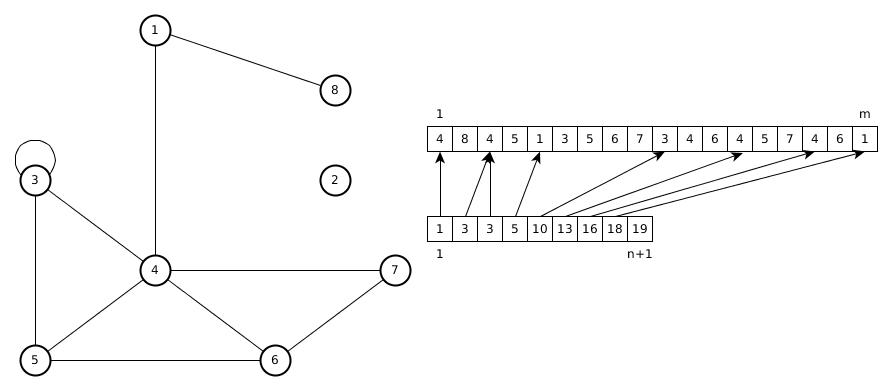
\includegraphics[width=0.9\textwidth]{graphrepresentation}
 	\caption{Zum Graphen werden die Kanten im oberen Array abgespeichert, sodass die Kanten von Knoten mit der Identifikationsnummer \(v+1\) neben den Kanten von Knoten mit der Identifikationsnummer \(v\) liegen. Um feststellen zu können, wo die Kanten des jeweiligen Knoten im Array beginnen, wird noch ein Hilfsarray benötigt, das zu jedem Knoten die Position abspeichert. Schlingen im Graphen werden nicht abgespeichert.}
	\label{fig:graphrepresentation}
\end{figure}
\subsection{Paralleler BFS mit Allreduce Kommunikation}
\label{sec:allreduce_details}
Wichtig für die Implementierung dieses Algorithmus ist, dass wir für das Array \lstinline{a[1..n]} und \lstinline{v[1..n/p]} aus Algorithmus~\ref{par_allvisited} eine sogenannte \textbf{\textit{Bitmap}} beziehungsweise ein Bit Array verwenden. Da bei diesen Arrays nur zwischen der Information 0 oder 1 unterschieden werden muss, ist hier ein Bit pro Knoten für diese Information ausreichend. Es wäre in Bezug auf den Speicher platzverschwendend, wenn man pro Knoten einen Speicher von mehreren Byte allokiert, nur damit man die Zahl 0 oder 1 abspeichert.\\
Deshalb wird bei einer \textit{Bitmap} wirklich jedes Bit eines Wertes vom Typ Integer ausgenutzt. In unserer Implementierung verwenden wir vorzeichenlose Integer mit einer Größe von 64 Bit. Damit können wir für jeden dieser Integer-Werte, in Bezug auf die Information 0 oder 1, genau 64 Knoten abdecken.\\
Ebenfalls maßgebend ist die Implementierung der Funktion \lstinline{GETNEWVISITED} aus Algorithmus~\ref{par_allvisited}, da diese eine wichtige Rolle in Bezug auf die Laufzeit des Algorithmus spielt. Schritt 1 zur Implementierung der Funktion \lstinline{GETNEWVISITED} ist die Verknüpfung des Bereichs des Arrays \lstinline{a[n/p*rank+1..n/p*(rank+1)}, also der Bereich für den der jeweilige Prozessor zuständig ist, mit dem Einerkomplement des Arrays \lstinline{v[1..n/p]} mittels binären Operation \lstinline{AND}. Mit \lstinline{n/p*rank+1} beziehungsweise \lstinline{n/p*(rank+1)} bekommt man den erforderlichen Start- und Endindex des Arrays \lstinline{a}, da jeder Prozessor für \(n/p\) Knoten verantwortlich ist und die Zuständigkeitsbereiche der Prozessoren geordnet nach dem Rang der Prozessoren im Array \lstinline{a} abgelegt sind. Das Ergebnis der \lstinline{AND} Verknüpfung ist nun wieder eine Bitmap der Länge \(n/p\), bei dem jene Knoten auf 1 gesetzt sind, die im letzten Level neu besucht wurden, jedoch noch nicht im aktuellen Level bearbeitet worden sind, also bei denen die Nachbarn im aktuellen Level besucht werden müssen. 
\begin{figure}[h]
 	\centering
	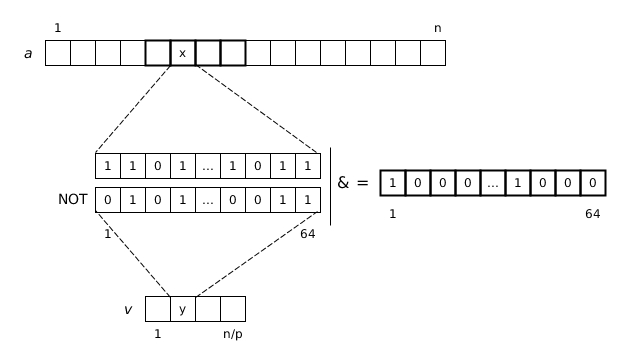
\includegraphics[width=0.7\textwidth]{getnewvisited}
 	\caption{Jeder Prozess arbeitet auf dem  selben Array \lstinline{a}, welches durch die Barrier-Synchronisation am Ende jedes Superschrittes synchron gehalten wird. Das Array \lstinline{v} unterscheidet sich jedoch, je nachdem welche Knoten, für die der Prozess zuständig ist, bearbeitet wurden. Außerdem muss jeder Prozess einen anderen Bereich des Arrays \lstinline{a} betrachten, was davon abhängt, welchen Rang der jeweilige Prozess hat. Dieses Beispiel zeigt einen Ausschnitt von der Funktion \lstinline{GETNEWVISITED} des Prozesses mit dem Rang 1, wobei in diesem Beispiel Ränge von 0 bis 3 vergeben wurden. Der Bereich \lstinline{a[5..8]} wird mit dem lokalen Array \lstinline{v} so verknüpft, dass eine Bitmap resultiert, die jene Knoten auf 1 gesetzt hat, die in diesem Level bearbeitet werden müssen.}
	\label{fig:getnewvisited}
\end{figure}
Abbildung~\ref{fig:getnewvisited} zeigt eine grafische Veranschaulichung dieser Implementierung der Funktion \lstinline{GETNEWVISITED}. In diesem Beispiel werden Arbeitsschritte des Prozesses mit dem Rang 1 gezeigt. Dieser arbeitet mit dem Bereich \lstinline{a[5..8]}, da das Array \lstinline{a} aus insgesamt 16 Feldern besteht und wir in diesem Beispiel davon ausgehen, dass es 4 arbeitende Prozesse gibt. Sowohl beim lokal gespeicherten Array \lstinline{v} als auch beim Array \lstinline{a} handelt es sich um Arrays von vorzeichenlosen Integer einer Größe von 64 Bit. Der Prozess muss über jedes der Felder vom Array \lstinline{a[5..8]} iterieren und mit dem korrespondierenden Feld des Arrays \lstinline{v} verknüpfen. In Abbildung~\ref{fig:getnewvisited} befindet sich der Prozess mit Rang 1 gerade auf dem zweiten der vier Felder, wobei es sich bei diesen Arrays um Bitmaps handelt, das heißt es wird in jedem dieser Felder die Information 0 oder 1 über insgesamt 64 Knoten gespeichert. Werden nun diese zwei Felder, in diesem Fall \lstinline{a[6]} mit dem Wert \lstinline{x} und das Einerkomplement von \lstinline{v[2]} mit dem Wert \lstinline{y}, mittels der binären Operation \lstinline{AND} verknüpft, erhalten wir ein Integer der Größe von 64 Bit, bei dem jene Bits beziehungsweise Knoten auf 1 gesetzt sind, die im letzten Level neu besucht, jedoch bis jetzt noch nicht bearbeitet wurden. Am Ende der \lstinline{GETNEWVISITED} Funktion erhalten wir eine Bitmap, die Informationen über 256 Knoten speichert und jene Bits oder Knoten auf 1 gesetzt hat, die in diesem Level noch bearbeitet werden müssen.\\
In Schritt 2 müssen nun genau diese Knoten aus dem berechneten Integer beziehungsweise der resultierenden Bitmap herausgefiltert werden, was der \lstinline{$\textbf{for}$} Schleife in Zeile 14 in Algorithmus~\ref{par_allvisited} entspricht. Dies ist auf verschiedene Wege möglich. Eine ineffiziente Variante wäre über alle Bits zu iterieren und zu prüfen, ob dieses auf 1 gesetzt ist. Mittels der aktuellen Position der Iteration kann man auf die Identifikationsnummer des Knoten schließen.\\
Wir haben uns für eine effizientere Variante entschieden, in dem wir davon ausgehen, dass eher wenige Knoten in der aus Schritt 1 resultierenden Bitmap auf 1 gesetzt sind, was besonders in Hinblick auf dünne Graphen der Fall ist. Wir machen Gebrauch von der in GCC (\textit{GNU Compiler Collection}) integrierten Funktion \lstinline{__builtin_clzll}, was der Funktion \lstinline{__builtin_clz} entspricht, nur dass sie auf Integer der Größe von 64 Bit operiert. Diese Funktion liefert die Anzahl der führenden Bits, die auf 0 gesetzt sind. Daraufhin kann auf die Position des Knoten geschlossen werden, der in der Bitmap aus Schritt 2 ausgehend vom höchstwertigen Bit in Richtung niedrigstwertigen Bit als nächstes auf 1 gesetzt ist, wobei man beachten muss, dass man mit dieser Funktion immer nur auf 64 Bit der Bitmap operieren kann. Damit liefert \lstinline{__builtin_clzll} mathematisch nichts anderes als den Logarithmus zur Basis 2 einer 64 Bit Zahl. Nachdem man die Position berechnet hat, wird der jeweilige Knoten bearbeitet und das Bit dieses Knoten auf 0 gesetzt. Schritt 2 wird solange wiederholt, bis alle Bits in der Bitmap auf 0 gesetzt sind.\\
Die Verwendung von Bitmaps hat nicht nur den Vorteil, dass man die Information über besucht oder nicht besucht effizienter abspeichern kann, sondern auch dass man innerhalb der \lstinline{ALLREDUCE} Operation des Arrays \lstinline{a} in Algorithmus~\ref{par_allvisited} weniger Daten zwischen den Prozessoren kommunizieren muss. In unserer Implementierung wird das bewerkstelligt durch die von MPI zur Verfügung gestellte Operation \lstinline{MPI_Allreduce} und der Bitmap, die für das Array \lstinline{a} steht. Weiters wichtig für diese Implementierung ist, dass jeder MPI Prozess auf genau einem Prozessor beziehungsweise Kern eines Prozessors der verwendeten DMM ausgeführt wird. DMMs bestehen aus mehreren Verarbeitungseinheiten (Knoten) und einem Verbindungsnetzwerk. Ein Knoten ist dabei ein selbständige Einheit, die aus einem oder mehreren Prozessoren beziehungsweise Prozessorkernen besteht. Damit ist es der Fall, dass wenn mehrere Kerne eines Prozessors verwendet werden, dass auch genauso viele MPI Prozesse darauf ausgeführt werden, die auch mittels \textit{Message Passing}, also MPI, miteinander interagieren beziehungsweise kommunizieren. Abbildung~\ref{fig:purempi} zeigt eine abstrakte Darstellung dieser Zuweisung von MPI Prozessen zu Prozessorkerne.
\begin{figure}[h]
    \centering
    \begin{subfigure}[b]{0.45\textwidth}
        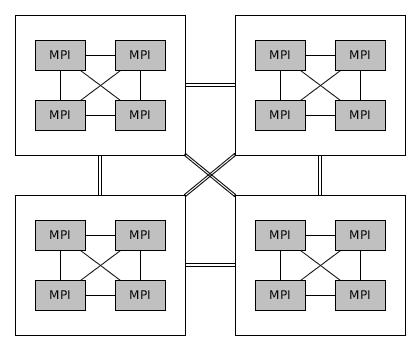
\includegraphics[width=1\textwidth]{purempi}
        \caption{MPI}
        \label{fig:purempi}
    \end{subfigure}
   \qquad
    \begin{subfigure}[b]{0.45\textwidth}
        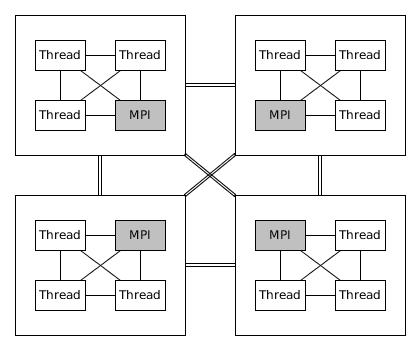
\includegraphics[width=1\textwidth]{hybridmasteronly}
        \caption{MPI + OpenMP}
        \label{fig:hybridmasteronly}
    \end{subfigure}
    \caption{Abbildung~\ref{fig:purempi} zeigt die Basisvariante des Algorithmus~\ref{par_allvisited}, bei der ausschließlich mittels MPI kommuniziert wird. Im Gegensatz dazu kommunizieren in Abbildung~\ref{fig:hybridmasteronly} nur die Master Threads per MPI, innerhalb eines Knoten operieren parallele Threads auf physikalisch gemeinsamen Speicher.}
\label{fig:normalandhybrid}
\end{figure}
\subsection{Hybrid-Variante mit Allreduce Kommunikation}
Bei den Hybrid-Varianten wird die Tatsache ausgenutzt, dass die Knoten der DMM Rechner mit physikalisch gemeinsamen Speicher (SMM - \textit{shared memory machine}) darstellen und deshalb eine Kommunikation mittels \textit{Message Passing} nicht unbedingt notwendig ist. Hier machen wir Gebrauch von parallel arbeitenden \textbf{Threads}, die auf einem Knoten der DMM ausgeführt werden. Wir führen also pro Knoten genau einen MPI Prozess aus und starten innerhalb dieses Knoten eine Vielzahl von Threads, die der Anzahl der Prozessorkerne entspricht. Die Threads führen dann explizit definierte parallele Bereiche aus. Abbildung~\ref{fig:hybridmasteronly} zeigt den gerade beschriebenen Sachverhalt, wodurch auch ein Vergleich zu Abbildung~\ref{fig:purempi} möglich wird.\\
In unserer Implementierung dieser Hybrid-Variante haben wir als parallelen Bereich die Zeilen von 12-20 aus Algorithmus~\ref{par_allvisited} gewählt. Dies entspricht der Funktion \lstinline{GETNEWVISITED} und der Iteration über die neue besuchten aber noch nicht bearbeiteten Knoten. Ein wichtiger Punkt dabei ist, dass es nicht möglich sein darf, dass mehrere Threads gleichzeitig die Bitmap \lstinline{a} verändern, da ein Feld dieses Arrays die Information über insgesamt 64 Knoten enthält und sonst falsche Werte in die Felder geschrieben werden, wenn mehrere Threads gleichzeitig auf dem selben Feld arbeiten. Eine Möglichkeit wäre einen kritischen Bereich über die Zeile 18 in  Algorithmus~\ref{par_allvisited} zu machen. Maßgebend für einen kritischen Bereich ist, dass nur ein Thread in diesen eintreten darf. In diesem Fall dürfen nicht mehrere Threads gleichzeitig in die \textit{Bitmap} \lstinline{a} schreiben. In unserer Implementierung haben wir uns aber für die Variante entschieden, dass jeder Thread eine lokale Kopie der Bitmap \lstinline{a} beim Eintreten in den parallelen Bereich von Zeile 12-20 erhält und auch jeder Thread nur seine lokale Kopie verändern beziehungsweise auslesen kann. Am Ende des parallelen Bereichs werden dann die lokalen Kopien aller Threads auf eine Bitmap wieder abgegleicht. Diese Variante ist auf jeden Fall die effizientere, da es nicht sein kann, dass die Threads gegenseitig auf sich warten, um in den kritischen Bereich eintreten zu dürfen.\\
In dieser Implementierung verfügt zwar jeder MPI Prozess, der einem Knoten der DMM zugewiesen ist, über einen größeren Teilgraphen \(G_{p}\) jedoch stehen diesem MPI Prozess mehrere Threads zur Abarbeitung dieses Teilgraphen zur Verfügung, die parallel ausgeführt werden. Diese Art von Vorgehensweise verfolgt den Ansatz eines \textit{$\textbf{Hybrid Masteronly}$} Programmiermodell, wie von Hager, Jost und Rabenseifner in \cite{hybrid} bezeichnet. Charakteristisch für dieses Programmiermodell ist, dass keine MPI Operationen innerhalb von parallelen Bereichen ausgeführt werden und dass während die Master Threads der Knoten mittels \textit{Message Passing} miteinander kommunizieren, alle anderen Threads inaktiv sind.\\
Wenn man diese Hybrid-Variante mit der normalen Variante aus Kapitel~\ref{sec:allreduce_details} vergleicht, ist es der Fall, dass bei der normalen Variante der Graph \(G\) auf die MPI Prozesse aufgeteilt wird und für jedes Level jeder MPI Prozess \(p\) sequentiell den Teilgraphen \(G_{p}\) durchsucht. Im Gegensatz dazu wird bei der Hybrid-Variante zwar ebenfalls der Graph auf die MPI Prozesse aufgeteilt, jeder MPI Prozess \(p\) durchsucht jedoch den Teilgraphen \(G_{p}\) parallel, je nach Anzahl der vorhandenen Threads.
\subsection{Paralleler BFS mit All-to-all Kommunikation}
Zu Beginn ist es wichtig, dass es sich bei dieser Implementierung um eine reine MPI Implementierung handelt. Jeder Prozess erhält dabei wie bei den vorangehenden Implementierungen \(n/p\) Knoten, für die er zuständig ist.\\
Um den Rang eines Prozessors beziehungsweise in unserem Fall eines MPI Prozesses per \lstinline{FIND_OWNER} in Algorithmus~\ref{par_alltoall} zu berechnen, ist es in unserer Implementierung ausreichend, die Identifikationsnummer des zu bestimmenden Knotens durch die Anzahl der Knoten zu dividieren, für die ein Prozess zuständig ist, und den Nachkommaanteil des Ergebnisses abzuschneiden beziehungsweise auf die nächste ganze Zahl abzurunden. Für die Datenstrukturen \lstinline{FS}, \lstinline{NS} und \lstinline{NS$_{p_{i}}$} werden Arrays vom Typ Integer verwendet, wobei es sich auch wieder um 64-Bit Integer handelt.\\
Um die \lstinline{ALLTOALL} Operation von Algorithmus~\ref{par_alltoall} in Zeile 31 zu realisieren, sind in unserer Implementierung zwei MPI Operationen notwendig, nämlich \lstinline{MPI_Alltoall} und \lstinline{MPI_Alltoallv}. Mittels \lstinline{MPI_Alltoall} wird zuerst zwischen den MPI Prozessen ausgetauscht, wie viele Knoten ein Prozess von den anderen Prozessen zu erwarten hat, damit dieser die Parameter für die Operation \lstinline{MPI_Alltoallv} vorbereiten kann, in der dann die eigentlichen Knoten ausgetauscht werden, die in der nächsten Iteration des Algorithmus abgearbeitet werden.\\
Ein weiteres Merkmal dieser Implementierung ist, dass es nicht ausreichend ist, nur die Identifikationsnummern der neu besuchten Knoten zwischen den Prozessen auszutauschen. Es muss zu jeden Knoten, der in der Datenstruktur \lstinline{NS$_{p_{i}}$} abgespeichert wird, auch der mögliche Vater gespeichert werden, also von dem aus der neu besuchte Knoten besucht wurde, damit der zuständige Prozess in der nächsten Iteration weiß, welchen Knoten er als Vater im Parent Array eintragen muss. Diese Information ist in Algorithmus~\ref{par_alltoall} als Attribut \lstinline{$\pi$} realisiert, wird jedoch in unserer Implementierung so abgespeichert, dass in allen Arrays zwei aufeinanderfolgende Felder eine Einheit bilden. Das erste Feld dieser Einheit speichert die Identifikationsnummer des neu besuchten Knotens, das zweite Feld speichert die Identifikationsnummer des Knotens, von dem aus der Knoten im ersten Feld besucht wurde. Es müssen also insgesamt \(2m\) 64-Bit Integer Werte durch die \lstinline{MPI_Alltoallv} Operation zwischen den MPI Prozessen ausgetauscht werden, wenn \(m\) Knoten innerhalb eines Levels von allen Prozessen neu besucht wurden.\\
Das Einsammlen der Teil-Parent Arrays wird durch die MPI Operation \lstinline{MPI_Gather} vom Prozess mit dem Rang \lstinline{$p_{0}$} durchgeführt.
\section{Analyse der Algorithmen und Versuchsergebnisse}
\label{sec:analysechapter}
\subsection{Analyse}
\label{sec:analyse}
Der nächste wichtige Schritt ist, die Algorithmen zu analysieren und bezüglich Laufzeit und Kosten mit dem sequentiellen Algorithmus~\ref{stacks} zu vergleichen. Dieser sequentielle Algorithmus stellt einen optimalen Algorithmus dar, es lässt sich also kein Algorithmus finden, der bezüglich Laufzeit der Breitensuche besser ist. In dieser Analyse werden wir das Akkumulieren oder Einsammeln des Parent Arrays außer Acht lassen, da wir davon ausgehen, dass ein verteiltes Parent Array ausreichend ist. \\
Genauso wie bei Algorithmus~\ref{stacks} die \lstinline{$\textbf{while}$} Schleife von Zeile 10-19 \($O$(H)\)-mal ausgeführt wird, wird diese auch in Algorithmus~\ref{par_allvisited}, was dem parallelen Algorithmus mit Allreduce Kommunikation entspricht, von Zeile 10-22 \($O$(H)\)-mal ausgeführt. \(H\) ist die Höhe des Breadth-First Trees. Es ist jedoch bei unserer Implementierung des Algorithmus~\ref{par_allvisited} nicht möglich, wie beim sequentiellen Algorithmus~\ref{stacks} in Zeile 11, in \(a\) Schritten, wenn \(a\) die Anzahl der neu besuchten Knoten in einem Level darstellt, über die neu besuchten Knoten eines Levels zu iterieren. Da die Information über neu besuchte beziehungsweise noch nicht bearbeitete Knoten in einer Bitmap mit \(n/p\) Feldern liegt, die der resultierenden Bitmap der Abbildung~\ref{fig:getnewvisited} entspricht, wobei \(n = |V(G)|\) und \(p\) die Anzahl der MPI Prozesse ist, müssen wir zumindest jeden Integer Wert, der sich durch die 64 Bits (Wortlänge \(w\)) eines Feldes der Bitmap ergibt, einmal überprüfen, ob sich in diesem ein neu besuchter, aber noch nicht bearbeiteter Knoten, befindet. Dies ist der Fall, wenn der Integer Wert größer als 0 ist. Dann weiß man, dass sich in diesem Wort der Bitmap zumindest ein Knoten befindet, der noch nicht bearbeitet wurde. Damit bekommt man rein für die Überprüfung in einem Level, ob es in den einzelnen Wörtern der Bitmap zumindest einen nicht bearbeiteten Knoten gibt, eine Laufzeit von \($O$(n/(wp))\) pro MPI Prozess. Im Beispiel der Abbildung~\ref{fig:getnewvisited} müssten also \(n/(wp) = 1024/(64*4) = 4\) Felder betrachtet werden, um zu überprüfen, ob zumindest ein Knoten dieses Prozesses in diesem Level bearbeitet werden muss. Summiert man diese Laufzeit über alle Levels der Breitensuche, ergibt sich eine Laufzeit für diese Überprüfung von \($O$(n/(wp)*H)\) pro MPI Prozess. Im Vergleich dazu, hat man bei der sequentiellen Implementierung eine Laufzeit von \($O$(n)\) in Bezug auf alle Levels der Breitensuche und dem Abarbeiten neu besuchter Knoten. Diese Laufzeit lässt sich auch zeigen, indem man zeigt, dass in den Levels \(1,2,3,..,d\) im sequentiellen Algorithmus \(a_{1},a_{2},a_{3},...,a_{d}\) Knoten besucht werden und \(a_{1} + a_{2} + a_{3} + ... + a_{d} \leq n\).\\
Falls ein Integer Wert der Bitmap größer als 0 ist, dieser also einen oder mehrere noch nicht bearbeitete Knoten beinhaltet, werden diese Knoten mithilfe der Funktion \lstinline{__builtin_clzll} herausgefiltert. Bei dieser Funktion nehmen wir eine Laufzeit von \($O$(1)\) an, dadurch kommt für einen Prozess zu den Kosten \($O$(n/(wp)*H)\) noch Kosten von \($O$(n/p)\) für das Herausfiltern mithilfe der Funktion \lstinline{__builtin_clzll} hinzu. Schließlich werden von jedem Prozess im Zuge der Abarbeitung der eigenen Knoten noch \($O$(m/p)\) Kanten betrachtet, wobei \(m = |E(G)|\). Daraus resultiert eine Gesamtlaufzeit für jeden Prozess von \($O$(n/p + m/p + n/(wp)*H)\), ohne jedoch die Laufzeit für die Kommunikationsoperation \lstinline{ALLREDUCE} miteinzuberechnen. Für \lstinline{MPI_Allreduce} muss man noch eine Laufzeit von \($O$(\log{p}+n/w)\) pro Level einplanen. Die Gesamtkosten \(C_{p}(n)\) der Implementierung des Algorithmus~\ref{par_allvisited} betragen damit \($O$(n + m + n/w*H + (\log{p}+n/w)*H) = \) \($O$(n + m + (n/w+\log{p})*H)\). Diese Implementierung ist also dann kostenoptimal, wenn die Höhe des Breadth-First Trees sehr viel kleiner ist als die Anzahl der Knoten im Graphen, also wenn gilt \(H \ll n\) und sollte auch auf solchen Graphen angewandt werden. Wann ein Graph diese Voraussetzung erfüllt, werden wir im Zuge der Versuchsergebnisse erklären.\\
Im Gegensatz dazu entstehen beim parallelen Algorithmus mit All-to-all Kommunikation, siehe dazu Algorithmus~\ref{par_alltoall}, genauso wie beim sequentiellen Algorithmus keine zusätzlichen Kosten für die Abarbeitung der Knoten aufgrund einer speziellen Datenstruktur, wie es durch die Bitmap in der Implementierung von Algorithmus~\ref{par_allvisited} der Fall ist. Aus diesem Grund ergibt sich für einen Prozess eine Laufzeit von \($O$(n/p)\) in Bezug auf die Abarbeitung aller neu besuchten Knoten in allen Levels, auch wenn wir davon ausgehen müssen, dass gewisse Knoten mehrmals zwischen den Prozessen durch die \lstinline{ALLTOALL} Operation kommuniziert und damit auch abgearbeitet werden, weil diese durch die Unwissenheit der Prozesse und durch unterschiedliche Kanten mehrmals besucht werden. Zu der Abarbeitung aller Knoten eines Prozesses in \($O$(n/p)\) kommt noch die Abarbeitung der zugehörigen Kanten hinzu. Diese wird mit einer Laufzeit von \($O$(m/p)\) durchgeführt, weshalb wir zu einer Gesamtlaufzeit von \($O$((n+m)/p)\) für Algorithmus~\ref{par_alltoall} ohne \lstinline{ALLTOALL} Operation kommen. Die Laufzeit für \lstinline{MPI_Alltoallv} wird mit \($O$(n+p)\) pro Level angenommen, wodurch die Gesamtkosten der Implementierung dieses Algorithmus \($O$(n + m + (n+p)*H)\) betragen. Es ist gut ersichtlich, dass dieser Algorithmus für Graphen in Bezug auf den sequentiellen Algorithmus kostenoptimal ist, wobei auch hier wieder der Breadth-First Tree aufgrund der \lstinline{MPI_Alltoallv} Operation eine geringe Höhe aufweisen muss.\\
Im nächsten Kapitel wird sich herausstellen, inwieweit sich die Laufzeit und die Kosten der Algorithmen beziehungsweise Implementierungen auf die Ausführungszeit und den Speedup auswirken. Es heißt nämlich nicht, dass die Algorithmen auch einen guten Speedup erzielen, selbst wenn die Voraussetzungen für Kostenoptimalität erfüllt sind.
\subsection{Versuchsergebnisse}
\label{sec:versuche}
In diesem Kapitel werden wir die vorgestellten Algorithmen beziehungsweise deren Implementierungen umfangreich auf der DMM Jupiter der TU Wien testen und vergleichen. Jupiter stellt 36 Knoten zur Verfügung, die jeweils zwei 8-Kern 2.3 GHz AMD Opteron 6134 Prozessoren besitzen und 32 GB Arbeitsspeicher zur Verfügung haben. Daraus resultieren insgesamt 576 Prozessorkerne und ein Arbeitsspeicher von 1152 GB. Die Knoten sind durch einen Infiniband QDR Switch MT4036 miteinander verbunden. Von diesen 576 Kernen werden wir bei unseren Versuchen maximal 512 Kerne nutzen, wobei wir darauf achten, dass so viele Knoten der DMM ausgelastet werden wie möglich, was einer Knotenanzahl von 32 entspricht. Wir werden wie Buluç und Madduri in~\cite{buluc} das Testmodell "'Flat MPI"' verfolgen, bei dem ein MPI Prozess pro verfügbaren Prozessorkern ausgeführt wird. Im Gegensatz dazu wird für die Implementierung der Hybrid-Variante vorerst folgendes Testmodell verfolgt, dass ein MPI Prozess pro Knoten der DMM gestartet wird und innerhalb des Knoten mehrere Threads parallel ausgeführt werden.\\
\begin{table}[H]
	\begin{tabular}{| l | l | l | l | m{4cm} |}
	\hline
	Abbildung & Anzahl Knoten & Anzahl Kanten & Eingabeparameter & Implementierungen\\ \hline
	Abbildung 8 & \(2^{22}\) & \(2^{26}\) & 0.57, 0.19, 0.19, 0.05 & {\lstinline!ALLREDUCE!}\linebreak{\lstinline!ALLREDUCE-HYBRID!}\linebreak{\lstinline!ALLTOALL!}  \\ \hline
	Abbildung 9 & \(2^{22}\) & \(2^{26}\) & 0.57, 0.19, 0.19 ,0.05 & {\lstinline!ALLTOALL!}\linebreak{\lstinline!ALLTOALL-VARIATION!} \\ \hline
	Abbildung 10 & \(2^{22}\) & \(2^{26}\) & 0.57, 0.19, 0.19, 0.05 & {\lstinline!ALLREDUCE!}\linebreak{\lstinline!REDUCE_SCATTER!} \\ \hline
	Abbildung 11 & \(2^{18}\) - \(2^{24}\)  & \(2^{22}\) - \(2^{28}\) & 0.57, 0.19, 0.19, 0.05 & {\lstinline!ALLREDUCE!}\linebreak{\lstinline!REDUCE_SCATTER!} \\ \hline
	\end{tabular}
	\caption{Zu sehen ist eine Übersichtstabelle der verwendeten Graphen innerhalb der Versuchsergebnisse. In Bezug auf die jeweiligen Abbildungen wird gezeigt, wie viele Knoten und Kanten der Graph hat, mit welchen Eingangsparametern dieser generiert wurde und welche Implementierungen auf diesem Graphen getestet wurden. Durch die gegebenen Eingangsparameter besitzen alle Graphen einen kleinen Durchmesser und dadurch kann auch der durch die Breitensuche entstehende Breadth-First Tree nur eine geringe Höhe aufweisen.}
	\label{tab:uebersicht}
\end{table}
Außerdem wichtig für die Auswertung der Ergebnisse ist der verwendete Graph und wie dieser generiert wurde. Wir haben uns für Stochastische Kronecker Graphen entschieden, die eine Generalisierung des \textit{recursive matrix} (R-MAT) Modells darstellen, da man mit diesem Modell sehr große Graphen schnell generieren kann und auch eine parallele Generierung überaus gut möglich ist. Diese erzeugten Graphen besitzen ebenfalls viele Eigenschaften von sogenannten \textit{real-networks}, die sich durch eine schiefe Knotengradverteilung auszeichnen. Das bedeutet, dass die meisten Knoten eines Graphen wenige ein- beziehungsweise ausgehende Kanten haben und nur ein kleine Anzahl an Knoten einen sogenannten hohen Knotengrad. Diese Informationen beziehen wir aus der Arbeit von Leskovec, Chakrabarti, Kleinberg, Faloutsos und Ghahramani~\cite{kronecker} und der Arbeit von Seshadhri, Pinar und Kolda~\cite{kronecker_study} und verweisen auch auf diese Arbeiten für ausführlichere Informationen, da dies sonst den Rahmen dieser Arbeit sprengen würde. Wir setzen die Werte in der Initiator Matrix, die für die Verteilung der Kanten im Graphen verantwortlich ist, genauso wie die Parameter \(a\), \(b\), \(c\) und \(d\) des R-MAT Generator auf \(0.57, 0.19, 0.19, 0.05\) um einen Graphen mit einem sehr kleinen Durchmesser(\(\leq 10)\)  und einer schiefen Knotengradverteilung zu erhalten. Der \textbf{Durchmesser} (\textit{diameter}) eines Graphen bezeichnet dabei die größte Distanz zwischen zwei beliebigen Knoten eines Graphen und hat auch direkten Einfluss auf die Höhe des \textit{Breadth-First Trees}, da diese nicht größer als der Durchmesser sein kann. Tabelle~\ref{tab:uebersicht} zeigt eine Übersicht über die verwendeten Graphen innerhalb unserer Versuchsergebnisse. Diese gibt Aufschluss darüber, welche Graphen bei den einzelnen Abbildungen verwendet wurden und welche Implementierungen innerhalb dieser Abbildungen getestet wurden.\\
Aufgrund dieser schiefen Knotengradverteilung käme es im Fall, dass wir den Graphen zur parallelen Breitensuche auf die MPI Prozesse aufteilen, zu einer ungleichmäßigen Lastverteilung zwischen den MPI Prozessen, was dazu führt das ein MPI Prozess für ein Level um einiges länger braucht als ein anderer MPI Prozess. Dies würde den Speedup, den wir durch unsere parallele Lösung erreichen wollen, um einiges verschlechtern. Deshalb führen wir eine Permutation der Identifikationsnummern der Knoten durch, was wir durch den \textbf{Fisher-Yates} Mischalgorithmus bewerkstelligen. Dies bewirkt, dass die Knoten mit hohen Knotengrad bezogen auf die Identifikationsnummer nicht knapp beieinander liegen, sondern gleichmäßig über alle Identifikationsnummern verteilt sind, damit sie auch gleichmäßig über die MPI Prozesse verteilt werden. Dies ist jedoch keine Garantie, dass wirklich jeder MPI Prozess gleich viele Kanten zugeordnet bekommt, auch wenn wir einen sehr guten Pseudozufallszahlengenerator verwendet haben, nämlich den Zufallsgenerator \textbf{KISS} (\textit{Keep it simple stupid}) entwickelt von Marsaglia und Zaman~\cite{kiss}. Außerdem ist es schwierig vorherzusagen, selbst wenn die MPI Prozesse gleich viele Kanten besitzen, wie viele und welche Knoten mit dazugehörige Kanten in jedem Level eines MPI Prozesses besucht werden.\\
Interessant ist noch die Validierung des Ergebnisses unserer parallelen Breitensuche. Vorgabe bei unseren Algorithmen ist immer, dass diese ein \textit{Parent Array} am Ende der Suche zur Verfügung stellen. Dabei gibt es verschiedene Möglichkeiten, wie man dieses \textit{Parent Array} auf Gültigkeit überprüft. Wir haben uns für eine relativ einfache Variante entschieden, indem das \textit{Parent Array} unserer parallelen Implementierung mit dem \textit{Parent Array} der sequentiellen Implementierung der Breitensuche verglichen und auf Richtigkeit geprüft wird, da wir davon ausgehen und es auch getestet haben, dass die sequentielle Implementierung korrekt arbeitet. Dazu wird jedes Feld des Arrays verglichen. Dabei kann der Fall eintreten, dass die Felder nicht übereinstimmen, was aber unter bestimmten Voraussetzungen erlaubt ist. Es ist bei der Implementierung von Algorithmus~\ref{par_allvisited} möglich, dass ein Kindsknoten im selben Level von mehreren Knoten, die aber von unterschiedlichen MPI Prozessen verwaltet werden, besucht wird und sich diese als Vater für diesen Knoten eintragen. Von dieser Auswahl an Vätern entscheiden wir uns bei der parallelen Lösung für den mit der höchsten Identifikationsnummer. Dieser muss aber nicht mit dem entsprechenden Vater in der sequentiellen Lösung übereinstimmen. Hier sind noch weitere Überprüfungen notwendig. Es muss nämlich geprüft werden, ob der eingetragene Vater der parallelen Lösung die selbe Distanz zum Startknoten beziehungsweise das gleiche Level wie der Vater aus der sequentiellen Lösung aufweist und ob dieser überhaupt mit dem Kindsknoten verbunden ist.\\
Als Compiler wurde der GNU C Compiler Version 4.4.7 und als MPI Implementierung wurde Open MPI Version 1.10.3 verwendet. Für die Kommunikation der Threads innerhalb eines Knoten im Falle der Hybrid Implementierungen haben wir die GNU OpenMP Bibliothek eingesetzt. Alle Tests haben wir auf 10 jeweils neu generierten Graphen durchgeführt. Jede angegebene Ausführungszeit ergibt sich aus dem Durchschnitt der Ergebnisse dieser Graphen. Eine Ausführungszeit beinhaltet 64 Durchläufe mit unterschiedlichen Startknoten und umfasst die Zeit von Beginn der Breitensuche bei bereits auf die Prozesse verteiltem Graphen bis zum Ende der Breitensuche, ohne dass jedoch das Parent Array akkumuliert oder eingesammelt wird. Jeder Startknoten muss dabei mindestens eine ein- beziehungsweise ausgehende Kante haben.\\
\begin{figure}[t]
	\centering
    \begin{subfigure}[h]{0.48\textwidth}
        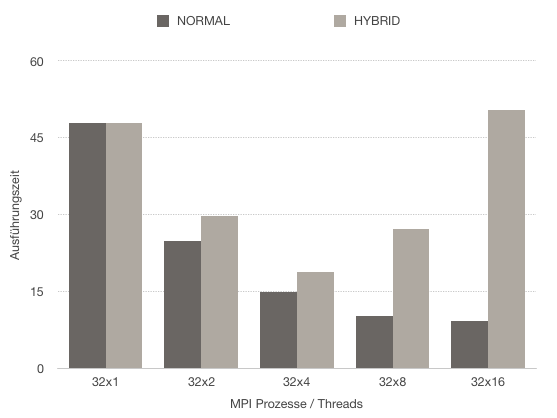
\includegraphics[width=1\textwidth]{times_algo1}
        \caption{Ausführungszeiten der Implementierungen von Algorithmus~\ref{par_allvisited}, reine MPI Implementierung und Hybrid, und von Algorithmus~\ref{par_alltoall}}
        \label{fig:times1}
    \end{subfigure}
   \hspace{0em}
    \begin{subfigure}[h]{0.48\textwidth}
        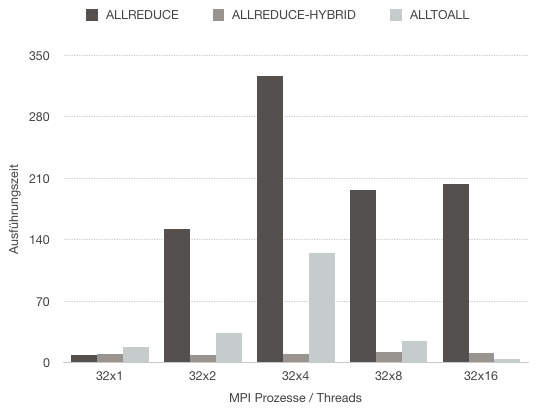
\includegraphics[width=1\textwidth]{reducing_parent}
        \caption{Dazugehörige Zeiten zum Akkumulieren beziehungsweise Einsammeln des \textit{Parent Arrays} per \lstinline{REDUCE}}
        \label{fig:reducing1}
    \end{subfigure}
    \caption{Diese Abbildungen zeigen die Ausführungszeiten unserer Implementierungen in Sekunden und die dazugehörigen Zeiten zum Kommunizieren des \textit{Parent Arrays} per \lstinline{REDUCE} Operation, innerhalb der \lstinline{ALLREDUCE}-Varianten, oder per \lstinline{GATHER} Operation, welche bei der \lstinline{ALLTOALL}-Variante notwendig ist, damit dieses dem Wurzelprozessor zur Verfügung steht, da die einzelnen MPI Prozesse nur Teile dieses \textit{Parent Arrays} befüllt haben.}
\label{fig:analyse1}
\end{figure}
Abbildung~\ref{fig:analyse1} zeigt die Ausführungszeiten unserer Implementierungen von Algorithmus~\ref{par_allvisited} und der Implementierung von Algorithmus~\ref{par_alltoall} in Sekunden. Dabei handelt es sich um die reine MPI Implementierung des Algorithmus mit Allreduce Kommunikation, der Hybrid-Variante dieses Algorithmus und der reinen MPI Implementierung des Algorithmus mit All-to-all Kommunikation. Wir arbeiten hierbei mit einem Graphen mit einer Knotenanzahl von \(2^{22}\) und einer Anzahl von ungerichteten Kanten von \(2^{26}\), was bedeutet, dass wir es mit einem dünnen Graphen zu tun haben. Die Implementierungen werden auf Jupiter ausgeführt, wobei die Bezeichnungen auf der x-Achse 32x1, 32x2, 32x4, 32x8, 32x16 bedeuten, dass wir auf 32 Knoten von Jupiter und auf einer variablen Anzahl von Prozessoren je Knoten arbeiten. Damit starten wir im höchsten Fall der reinen MPI Implementierungen 512 MPI Prozesse, bei der Hybrid-Variante werden 32 MPI Prozesse gestartet, aber unterschiedlich viele Threads in jedem dieser MPI Prozesse. Auf der y-Achse des Diagramms ist die Zeit in Sekunden eingetragen.\\
Die Ausführungszeit der sequentiellen Implementierung \(T^{*}(n)\) beträgt \(376,97\) Sekunden. Dadurch beträgt der Speedup bei der reinen MPI Variante mit Allreduce Kommunikation im Fall von 512 MPI Prozessen \(S_{512} = 36,99\). Es ist in Abbildung~\ref{fig:times1} ersichtlich, dass durch Verdopplung der MPI Prozesse eine deutlich schnellere Abarbeitung der Breitensuche möglich ist. Außer beim Sprung von 256 auf 512 MPI Prozessen konnte bei der reinen MPI Variante mit Allreduce Kommunikation eine nur minimal kürzere Ausführungszeit erreicht werden, was bedeutet dass der Speedup von 256 und 512 involvierten MPI Prozessen fast gleich ist. Im Vergleich dazu erreicht die Hybrid-Variante einen ähnlichen Speedup bis zu einer Anzahl von 4 arbeitenden Threads pro Knoten, kann jedoch dann bei Erhöhung der Threadanzahl nicht mehr mithalten, was damit zu tun hat, dass die Threads zu lange brauchen, um die lokalen Kopien der Bitmap \lstinline{a} zu akkumulieren. Vergleicht man dazu die Ausführungszeiten der Implementierung des Algorithmus mit All-to-all Kommunikation ist ein deutlich schlechterer Speedup gegenüber der reinen MPI Implementierung des Algorithmus mit Allreduce Kommunikation zu erkennen, obwohl dieser anhand der Analyse in Kapitel~\ref{sec:analyse} eigentlich einen guten Eindruck in Bezug auf die Laufzeit gemacht hat und wir uns auch schnellere Ausführungszeiten erwartet hätten. Der Speedup beträgt hier im besten Fall bei 64 MPI Prozessen \(S_{64} = 8,24\). Das schlechtere Abschneiden dieser Implementierung liegt einerseits an der \lstinline{ALLTOALL} Operation, da diese äußerst aufwendig ist und zu einem Flaschenhals führen kann, überhaupt bei großen Datenmengen und anderseits an dem Fakt, dass bereits bearbeitete Knoten mehrmals mittels der \lstinline{ALLTOALL} Operation ausgetauscht werden und überprüft werden müssen, da die Prozesse nur beschränkt die Information besitzen, ob Knoten, für die andere Prozesse zuständig sind, bereits besucht wurden und deshalb den zuständigen Prozess bei Besuch des Knotens informieren müssen. Außerdem muss man bei dieser Variante auch miteinberechnen, dass nicht nur die reine \lstinline{MPI_Alltoallv} Operation eine Rolle für den höheren Aufwand spielt, sondern auch die Vorbereitungen dazu, dass überhaupt die richtigen Knoten mittels der \lstinline{MPI_Alltoallv} Operation ausgetauscht werden. Zu diesen Vorbereitungen zählt zum Beispiel eine \lstinline{MPI_Alltoall} Operation, damit jeder Prozess weiß, wie viel Speicher für die folgende \lstinline{MPI_Alltoallv} allokiert werden muss.\\
Interessant sind weiters die Zeiten für das Akkumulieren beziehungsweise Einsammeln des \textit{Parent Arrays}. Zu sehen in Abbildung~\ref{fig:reducing1}, ist die Dauer des Akkumulieren der reinen MPI Implementierung mit Allreduce Kommunikation im Fall 32x1 relativ gering. Jedoch mit steigender Anzahl von MPI Prozessen, die an der Akkumulationsoperation beteiligt sind, geht die Dauer der Operation extrem in die Höhe und übertrifft, im Fall 32x4 mit 326.62 Sekunden, sogar fast die Ausführungszeit der Breitensuche der sequentiellen Variante. Der Vorteil der Hybrid-Variante ist, da immer 32 MPI Prozesse beteiligt sind, die Dauer der Akkumulation immer gleich gering bleibt. Im Gegensatz dazu ist die Ausführungszeit für das Einsammeln der Teil-Parent Arrays bei der All-to-all-Implementierung um einiges geringer als bei der reinen MPI Implementierung mit Allreduce Kommunikation und ist sogar im Fall 32x16 doppelt so schnell wie die Hybrid-Variante. \\
Jedoch spielt die Dauer der Akkumulation oder Einsammeln des Parent Arrays nicht so eine große Rolle, da es für uns ausreichend ist, wenn das Parent Array verteilt auf den MPI Prozessen liegt. Abbildung~\ref{fig:reducing1} sollte aber zeigen, wie teuer diese Operation bei steigender Anzahl von MPI Prozessen sein kann. Ausgehend von diesen Ergebnissen, haben wir Tests der Implementierung der Hybrid-Variante von Algorithmus~\ref{par_allvisited} durchgeführt, bei denen wir ausgehend von 4 Threads die Anzahl der MPI Prozesse variiert haben, da in Abbildung~\ref{fig:times1} im Fall von 4 parallel arbeitenden Threads der beste Speedup der Hybrid-Variante erreicht wurde. Wir sind also vom ursprünglichen Testmodell abgewichen, bei dem wir pro Knoten der DMM nur einen MPI Prozess ausführen. Im Fall von 128 gestarteten MPI Prozessen und jeweils 4 Threads zu jedem dieser MPI Prozesse konnte eine sehr ähnliche Ausführungszeit wie bei der reinen MPI Implementierung mit Allreduce Kommunikation erreicht werden, wodurch sich ein Speedup von \(S_{512} = 33,74\) ergeben hat. Die Zeit für das Akkumulieren des Parent Arrays ist jedoch genauso hoch wie im Fall 32x4 der normalen Variante.\\
\begin{figure}[h]
 	\centering
	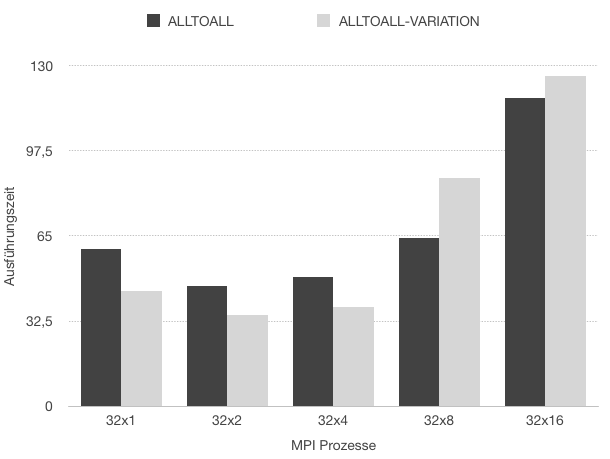
\includegraphics[width=0.7\textwidth]{alltoall_variation}
 	\caption{Zu sehen sind die Ausführungszeiten der ursprünglichen Implementierung der All-to-all-Variante und der abgeänderten Version. Bis zu einer Anzahl von 128 MPI Prozesse ist die abgeänderte Variante schneller, bei einer Anzahl von 256 und 512 MPI Prozessen ist sie jedoch um ein kleines Stück langsamer.}
	\label{fig:alltoall_change}
\end{figure}
Zusätzlich haben wir noch eine Änderung der Implementierung der Variante mit All-to-all Kommunikation vorgenommen. Die Implementierung, die auch in Abbildung~\ref{fig:analyse1} getestet wurde, beinhaltet die Vorgehensweise, dass jeder Prozessor beziehungsweise Prozess eine lokale Bitmap über alle Knoten besitzt, in der abgespeichert wird, welche Knoten von diesem Prozess aus bereits besucht worden sind. Da dies zwar bewirkt, dass ein Knoten vom selben Prozess nicht zwei mal besucht wird, aber mehr Arbeitsaufwand verursacht, haben wir die Implementierung so abgeändert, dass diese Überprüfung nicht mehr stattfindet und präsentieren in Abbildung~\ref{fig:alltoall_change} die Ergebnisse dazu. Es ist zu erkennen, dass der Aufwand um so eine lokale Überprüfung durchzuführen doch höher ist, als einfach die Knoten ungeprüft zu den jeweiligen verantwortlichen Prozessen zu schicken. Dies trifft zumindest für eine Prozessanzahl bis 128 zu, wo ein Speedup bei 64 MPI Prozessen von \(S_{64} = 10,86\) erreicht wurde, darüber kann die Basisvariante Zeit gewinnen, auch wenn dies nicht zu vergleichen ist mit den Ausführungszeiten und Speedups der Allreduce-Varianten.
\subsection{Distanz Array statt Parent Array}
\label{sec:distanzarray}
In vielen Anwendungen ist es ausreichend, dass man am Ende der Breitensuche anstelle eines Breadth-First Trees die Distanzen ausgehend vom Wurzelknoten zu den erreichten Knoten in Form eines \textbf{Distanz Array} zur Verfügung stellt beziehungsweise ausgibt. Es wird also das durch die Breitensuche ermittelte Level des Knoten im Distanz Array abgespeichert.\\
Aufgrund der Tatsache, dass es aufwändiger ist, einen Breadth-First Tree am Ende der Breitensuche zu erzeugen, werden wir in diesem Kapitel eine Variante von Algorithmus~\ref{par_allvisited} vorstellen, die ein Distanz Array am Ende ausgibt, und dadurch auch schneller arbeitet als der Algorithmus, der ein Parent Array erzeugen muss. Ein großer Unterschied dieser Variante ist, dass die Prozessoren nicht die Information besitzen müssen, welche Knoten des Graphen in den bisherigen Iterationen beziehungsweise Superschritten besucht worden sind, was bei Algorithmus~\ref{par_allvisited} mit der Bitmap \lstinline{a} gewährleistet ist.  Diese Information war nur in Bezug auf das Parent Array notwendig, damit sich ein Knoten als Vater eines anderen Knoten im Parent Array einträgt, falls dieser andere Knoten zuvor noch nicht besucht wurde, also in der synchronisierten Bitmap \lstinline{a} den Wert 0 aufweist.\\
In dieser Variante verfügen alle Prozessoren zu Beginn jedes Superschritts über eine lokale Bitmap über alle Knoten, die auf 0 initialisiert ist. Falls neue Knoten innerhalb des Superschritts besucht werden, setzt der zuständige Prozessor die neu besuchten Knoten in der lokalen Bitmap auf 1. Der Unterschied dieser Bitmap zur Bitmap \lstinline{a} in Algorithmus~\ref{par_allvisited} ist also, dass diese nicht wiedergibt, welche Knoten in allen Superschritten zuvor besucht wurden, sondern welche Knoten im aktuellen Superschritt neu besucht wurden. Nun ist es am Ende des Superschritts nicht notwendig, die Bitmaps der Prozessoren per \lstinline{ALLREDUCE} Operation zu synchronisieren. Hierbei würde jeder Prozessor eine Bitmap als Ergebnis der \lstinline{ALLREDUCE} Operation erhalten, die über alle Knoten des Graphen die Information besitzt, ob ein Knoten im aktuellen Superschritt besucht wurde oder nicht. Es ist jedoch für einen Prozessor nur notwendig, den Teil der Bitmap zu erhalten, der die Knoten enthält, für die der Prozessor zuständig ist. Dies lässt sich mit einer sogenannten \lstinline{REDUCE_SCATTER} Operation bewerkstelligen, welche von MPI durch die Operation \lstinline{MPI_Reduce_scatter} zur Verfügung gestellt wird. Diese funktioniert folgendermaßen, dass zuerst eine Einzelakkumulationsoperation über die lokalen Bitmaps der Prozessoren ausgeführt wird und danach diese akkumulierte Bitmap über die Prozessoren verteilt wird. In unserer Implementierung wird die Bitmap in gleich große Teile zerlegt und jeder Prozess erhält den Teil, der die Knoten enthält, für die dieser zuständig ist.\\
Im nächsten Superschritt werden die neu besuchten Knoten genauso behandelt beziehungsweise aus der Bitmap herausgefiltert wie in der Implementierung von Algorithmus~\ref{par_allvisited}. Im Gegensatz wird jedoch bei einem neu besuchten und nicht bearbeiteten Knoten die Distanz im lokalen Distanz Array abgespeichert. Da jeder Prozessor ein Distanz Array über die Knoten besitzt, für die er zuständig ist, wird dieses noch am Ende des Algorithmus per \lstinline{GATHER} Operation vom Prozessor mit dem Rang \lstinline{$p_{0}$} eingesammelt. Zur Analyse dieser Variante lässt sich sagen, dass diese die selben Gesamtkosten wie Algorithmus~\ref{par_allvisited} hat, jedoch kann man annehmen, dass \lstinline{MPI_Reduce_scatter} schneller abgearbeitet ist als \lstinline{MPI_Allreduce}, da im Gegensatz zu dieser nicht jeder Prozess eine Einzelakkumulationsoperation ausführen muss. Validiert wurde das Distanz Array der parallelen Implementierung folgendermaßen, dass dieses mit dem der sequentiellen Implementierung verglichen wurde.\\
\begin{figure}[h]
 	\centering
	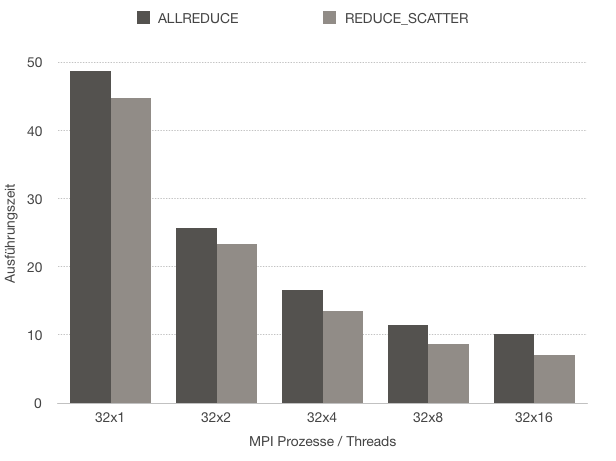
\includegraphics[width=0.7\textwidth]{reduce_scatter}
 	\caption{In allen Fällen erzielt die Reduce-Scatter-Variante eine bessere Ausführungszeit als die reine MPI Implementierung mit Allreduce Kommunikation. Dadurch kann auch ein besserer Speedup erzielt werden. Dieser beträgt bei 512 MPI Prozessen \(S_{512} = 53,93\).}
	\label{fig:reduce_scatter}
\end{figure}
Abbildung~\ref{fig:reduce_scatter} zeigt die Ausführungszeiten dieser Variante im Vergleich zur reinen MPI Implementierung des Algorithmus mit Allreduce Kommunikation, also der Implementierung, die sehr ähnlich zur dieser ist, nur dass diese am Ende ein Parent Array als Ausgabe erzeugt und deshalb eine \lstinline{ALLREDUCE} Operation zur Synchronisation benötigt. Die Ausführungszeiten beinhalten nicht das Einsammeln beziehungsweise Akkumulieren des Distanz oder Parent Arrays. Auch hier arbeiten wir mit einem Graphen mit einer Knotenanzahl von \(2^{22}\) und einer Anzahl von ungerichteten Kanten von \(2^{26}\), also den gleichen Graphen wie bei den vorhergehenden Versuchsergebnissen. Der erreichte Speedup der Reduce-Scatter-Variante ist deutlich höher und beträgt \(S_{512} = 53,93\). Die Zeit für das Einsammeln des Distanz Arrays bei einer Prozessanzahl von 512 mit 4,5 Sekunden ist hierbei auch deutlich geringer als das Akkumulieren des Parent Arrays mit fast über 200 Sekunden.
Darauf aufbauend haben wir die Reduce-Scatter-Variante im Vergleich zur Allreduce-Variante genauer getestet und diese auf Graphen mit unterschiedlicher Knotenanzahl ausgeführt, ebenfalls mit jeweils 64 Durchläufen. Diese Graphen erfüllen die gleichen Kriterien (Knotengradverteilung, Durchmesser,...) wie die für die vergangenen Tests verwendeten Graphen. Das Verhältnis zwischen Knoten und Kanten bleibt das gleiche. Dabei vergleichen wir den Speedup, den wir bereits von Abbildung~\ref{fig:reduce_scatter} kennen, mit den Speedups dieser zwei Implementierungen ausgeführt auf Graphen mit einer Knotenanzahl von \(2^{18}\) bis \(2^{24}\). Dabei ist ersichtlich, dass umso größer die Skalierung des Graphen wird, umso höher fällt der Speedup aus. Im Fall des Graphen von \(2^{24}\) Knoten konnte sogar bei der Reduce-Scatter-Variante ein Speedup von \(S_{512} = 72,30\) erreicht werden. Versuche auf noch größeren Graphen konnten leider nicht durchgeführt werden, da dies einfach schon zu viel Zeit beansprucht hat. Schon rein ein Test der sequentiellen Implementierung der Breitensuche auf einen Graphen mit einer Knotenanzahl von \(2^{24}\) hat ca. 25 Minuten gedauert. Abbildung~\ref{fig:speedups_reduce_scatter} zeigt den Anstieg des Speedups bei immer größer werdender Graphengröße und gleich bleibender Anzahl von 512 MPI Prozessen.
\begin{figure}[h]
 	\centering
	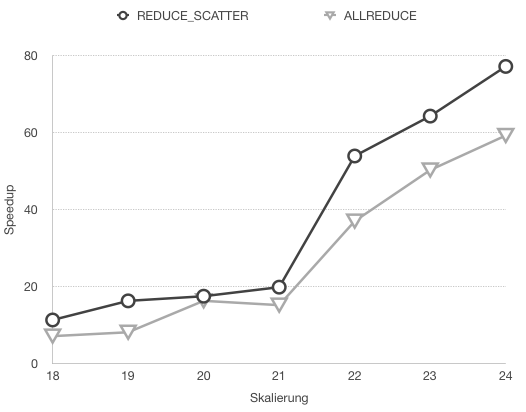
\includegraphics[width=0.6\textwidth]{speedups}
 	\caption{Diese Abbildung zeigt den Verlauf des Speedups der Reduce-Scatter- und der Allreduce-Variante bei steigender Knotenanzahl. Es ist zu sehen, dass dieser mit wachsender Knotenanzahl steigt und einen besonders großen Sprung von \(2^{21}\) auf \(2^{22}\) Knoten aufweist. }
	\label{fig:speedups_reduce_scatter}
\end{figure}
\section{Das Graph500 Projekt}
\label{sec:graph500}
Die Grundidee, warum das Graph500 Projekt, beschrieben durch Murphy, Wheeler, Barrett und Ang in \cite{graph500}, ins Leben gerufen wurde, ist die, dass es lange Zeit keine vernünftigen Benchmarks gegeben hat, die testeten, wie gut ein Hochleistungsrechner mit datenintensiven Anwendungen umgehen kann. Im Zuge dieses Projekts haben 50 internationale HPC (\textit{High Performance Computing}) Experten zusammengearbeitet, um gerade diese Lücke, die es im Bereich der Benchmarks gegeben hat, zu füllen und diese Art von Anwendungen abdeckt. Dadurch soll auch das zukünftige Design von Hardware Architekturen und Softwaresystemen, die solche Probleme lösen sollen, beeinflusst werden. Eine weitere überaus wichtige Eigenschaft dieses Benchmarks ist, dass die Resultate dieses Benchmarks auch Aufschluss über die Lösung vieler sogenannter \textit{Real World}-Probleme geben und wie schnell ein Hochleistungsrechner diese Probleme lösen könnte. Bereiche, in denen riesige Datenmengen durchsucht werden müssen, sind zum Beispiel \textit{Cybersecurity}, Medizinische Informatik (Datensätze von Patienten) und \textit{Social Networks}.\\
Aufgrund der Tatsache, dass die Breitensuche bei groß angelegten Graphen ebenfalls ein datenintensives Problem darstellt, steht diese im Mittelpunkt dieses Projekts, weshalb wir uns in dieser Arbeit diesem Projekt widmen und erläutern wie dieser Benchmark funktioniert beziehungsweise aufgebaut ist. Der Benchmark weist folgende Struktur beziehungsweise Ablauf auf:
\begin{enumerate} 
\item{Generieren der Kantenliste.}
\item{Die Kantenliste in eine geeignete Datenstruktur bringen, damit diese für die nächsten Schritte verwendet werden kann. (\textbf{Kernel 1})}
\item{Generieren von 64 (pseudo-)zufällig gewählten Startknoten für die darauf folgende Breitensuche.}
\item{Für jeden Startknoten:}
\begin{itemize}
         \item Durch die Breitensuche das Parent Array berechnen.  (\textbf{Kernel 2})
         \item Validieren des Parent Arrays.
      \end{itemize}
\item{Ausgabe von Leistungsinformationen.}
\end{enumerate}
Im ersten Schritt des Benchmarks werden die Kanten des Graphen generiert, wobei hier als Eingabe die Anzahl der Knoten und ungerichteten Kanten erwartet wird. Dabei werden Tupel von Knoten mit Hilfe eines Pseudozufallszahlengenerators generiert. Von der Spezifikation des Benchmarks wird erwartet, dass die Tupeln mithilfe eines Kronecker Generator generiert werden sollen. Dabei sollen die gleichen Parameter zur Generierung verwendet werden wie bereits bei unseren Graphen der vorherigen Versuchsergebnisse. Mehrfachkanten und Schlingen sind erlaubt. Es sollten in keinster Weise die Tupeln so generiert werden, dass der nächste Schritt (\textbf{Kernel 1}) einen Vorteil daraus schöpfen könnte. Im nächsten Schritt geht es darum, dass die Tupeln in eine Form beziehungsweise Datenstruktur gebracht werden, damit die Breitensuche durchgeführt werden kann. Möglichkeiten einen Graphen abzuspeichern, wurde bereits in Kapitel~\ref{sec:graphrepresentation} über Graphrepräsentationen vorgestellt. Dieser Punkt ist ein sehr wichtiger, da von diesem alle weiteren Schritte abhängen und den ganzen Benchmark beeinflussen. Deshalb ist dieser auch der erste Kernel des Benchmarks und wird bewertet, indem die Zeit der Transformation von der Liste von Tupeln zur entsprechenden Datenstruktur gestoppt wird.
Schritt 3 generiert 64 (pseudo-)zufällige unterschiedliche Startknoten, die zumindest eine ein- beziehungsweise ausgehende Kante besitzen. In Schritt 4 beginnt der Hauptteil des Benchmarks. Hier wird ausgehend von jedem generierten Startknoten die Breitensuche durchgeführt und als Ausgabe ein Parent Array erwartet. Die Breitensuche für alle 64 Startknoten mit zugehöriger Ausgabe wird als \textbf{Kernel 2} bezeichnet und wird ebenfalls innerhalb des Benchmarks bewertet. Es wird die Zeit für das Suchen ausgehend von den 64 Startknoten gemessen und dabei auch die Anzahl der besuchten Kanten innerhalb der Breitensuche gezählt, welche notwendig ist, um die Leistung der Implementierung und der Hardware in der Maßeinheit TEPS (\textit{traversed edges per second}) zu berechnen, also die Anzahl der besuchten Kanten pro Sekunde. Im vierten Schritt werden auch die berechneten Parent Arrays der einzelnen Durchläufe auf Richtigkeit geprüft. Dabei werden von der Spezifikation des Benchmarks fünf Kriterien genannt, die das Parent Array beziehungsweise der Breadth-First Tree erfüllen muss. Zu den Kriterien gehört zum Beispiel, dass überprüft werden muss, dass sich keine Zyklen im Breadth-First Tree befinden dürfen und dass Kanten innerhalb dieses Breadth-First Trees nur Knoten verbinden, die sich um genau ein Level unterscheiden. Diese Validierung wird jedoch nicht innerhalb des Benchmarks bewertet und ist nur dazu da, dass garantiert wird, dass die Implementierung der Breitensuche korrekt arbeitet.\\
Im fünften und letzten Schritt werden die Leistungsinformationen berechnet und ausgegeben. Dazu gehört die gemessene Zeit von \textbf{Kernel 1} und Informationen, die aus \textbf{Kernel 2} gewonnen werden konnten, wie zum Beispiel die gemessene Zeit für diesen Kernel und die Anzahl der besuchten Kanten pro Sekunde (TEPS).\\
Innerhalb dieser Arbeit haben wir versucht uns so weit wie möglich an das Schema des Graph500 Benchmarks zu halten, weshalb bei der Einsicht in unsere Implementierungen auch auffallen wird, dass die Implementierung in die einzelnen Kernel unterteilt ist. Ebenfalls haben wir auch zuerst die Tupelliste für einen Graphen generiert, der einen Stochastische Kronecker Graphen widerspiegelt und dann diese Tupelliste in unsere verwendete Datenstruktur überführt. Darauf aufbauend haben wir außerdem für unsere Messungen beziehungsweise Tests immer 64 Durchläufe vorgenommen, wobei jeder Startknoten eines Durchlaufes einen Knotengrad von mindestens 1 aufweisen muss. Damit hat das Graph500 großen Einfluss auf den Aufbau unserer Arbeit ausgeübt. Wir haben jedoch nicht die Anzahl der besuchten Kanten pro Sekunde berechnet, weshalb wir nicht die gleichen Leistungsinformationen ausgeben wie beim Graph500 Projekt.
\section{Fazit und weiterführende Arbeit}
\label{sec:fazit}
Abschließend zu dieser Arbeit lässt sich sagen, dass die Parallelisierung der Breitensuche eine herausfordernde Aufgabe darstellt, da sich diese irregulär bezüglich der Speicherzugriffe verhält. Das bedeutet, dass man nicht wirklich vorhersagen kann, welche Knoten durch die Breitensuche besucht werden und auf welche Speicheraddressen als nächstes zugegriffen wird. Natürlich hängt auch die Leistung des parallelen Algorithmus davon ab, was man sich von der Breitensuche als Ausgabe erwartet. Benötigt man einen Breadth-First Tree, sind mehr Operationen innerhalb der Breitensuche notwendig, was zu einer längeren Ausführungszeit beziehungsweise zu einem geringerem Speedup führt. Wir haben auch gesehen, dass mit steigender Größe der Datenmenge bessere Ergebnisse im Vergleich zur sequentiellen Variante erzielt werden konnten, was bei  sogenannten "'\textit{big data}"' Anwendungen unerlässlich ist. Am Ende dieser Arbeit haben wir uns noch mit dem Graph500 Projekt befasst. Mit diesem Projekt wollen wir uns in Zukunft noch näher beschäftigen und unsere Implementierungen mit Hilfe der Maßeinheit TEPS testen, womit ein Vergleich mit anderen Arbeiten besser möglich ist.\\
Außerdem wollen wir als weiterführende Arbeit einen Algorithmus entwickeln, der auf zweidimensionaler Zerlegung des Graphen beruht und herausfinden, welche Unterschiede und Herausforderungen im Vergleich zur eindimensionalen Zerlegung entstehen. Weiters sind Hybrid-Algorithmen ein interessantes Thema, weshalb wir für die reine MPI Implementierung mit All-to-all Kommunikation noch eine Hybrid-Variante entwickeln wollen, um zu sehen inwieweit sich hier Verbesserungen erzielen lassen, da die reine MPI Implementierung keine guten Ergebnisse erzielt hat.
\clearpage
\bibliographystyle{abbrv}
\bibliography{bachelor}
\clearpage
\appendix
\section{BFS Implementierungen}
\label{sec:versions}
\lstinputlisting[firstline=211,lastline=290,caption={Parallele Breitensuche mit Allreduce Kommunikation - MPI Only},label=mpionly_allreduce]{../Source/bfs_par_allvisited_parallelsort_improvement.c}
\lstinputlisting[firstline=219,lastline=307,caption={Parallele Breitensuche mit Allreduce Kommunikation - MPI + OpenMP},label=hybrid_allreduce]{../Source/bfs_hybrid.c}
\section{Source Code - graph500}
\label{sec:sourcecode}
\lstinputlisting[caption={graph500 - Breitensuche Implementierung },label=bfs]{../Source/bfs_par_allvisited_parallelsort_improvement.c}
\clearpage
\lstinputlisting[caption={Kronecker Generator},label=kronecker_generator]{../Source/kronecker_generator_par.c}
\clearpage
\lstinputlisting[caption={project.h},label=project]{../Source/project.h}

\clearpage


\end{document}